\documentclass[11pt,a4paper]{article}
\usepackage{times,latexsym}
\usepackage{url}
\usepackage[T1]{fontenc}
\usepackage{grffile}

\usepackage{CJKutf8}
\usepackage{fullpage}

\usepackage{tikz-dependency}

\newcommand\BibTeX{B{\sc ib}\TeX}
\newcommand\confname{EMNLP-IJCNLP 2019}
\newcommand\conforg{SIGDAT}

\usepackage{longtable}

\usepackage{amsmath}
\usepackage{tikz-dependency}
\DeclareMathOperator*{\argmax}{arg\,max}
\DeclareMathOperator*{\argmin}{arg\,min}
\DeclareMathOperator{\E}{\mathop{\mathbb{E}}}

\usepackage{amssymb}% http://ctan.org/pkg/amssymb
\usepackage{pifont}% http://ctan.org/pkg/pifont
\newcommand{\cmark}{\ding{51}}%
\newcommand{\xmark}{\ding{55}}%


\newcommand{\Prob}{\mathbb{P}}%

%\usepackage{pslatex}
%\usepackage{latexsym}
\usepackage[english]{babel}
\usepackage[utf8]{inputenc}
\usepackage{bm}
\usepackage{graphicx}
\usepackage{tikz}
\usepackage{xcolor}
\usepackage{url}
%\usepackage[colorinlistoftodos]{todonotes}
\usepackage{rotating}
\usepackage{multirow}



\newcommand{\japanese}[1]{\begin{CJK}{UTF8}{min}#1\end{CJK}}


\usepackage[T1]{fontenc}

\usepackage{pslatex}
%\usepackage{latexsym}
\usepackage[english]{babel}
\usepackage[utf8]{inputenc}
\usepackage{amsmath}
\usepackage{bm}
\usepackage{graphicx}
\usepackage{tikz}
\usepackage{xcolor}
\usepackage{url}
%\usepackage[colorinlistoftodos]{todonotes}
\usepackage{rotating}
%\usepackage{natbib}
\usepackage{amssymb}



\usepackage{natbib}
\bibliographystyle{unsrtnat}

\usepackage{amsthm}
 

\allowdisplaybreaks

\newcounter{theorem}
\newtheorem{proposition}[theorem]{Proposition}
\newtheorem{corollary}[theorem]{Corollary}
\newtheorem{question}[theorem]{Question}
\newtheorem{example}[theorem]{Example}
\newtheorem{defin}[theorem]{Definition}
\newtheorem{remark}[theorem]{Remark}
\newtheorem{lemma}[theorem]{Lemma}
\newtheorem{thm}[theorem]{Theorem}


\newcommand{\R}[0]{\mathbb{R}}
\newcommand{\Ff}[0]{\mathcal{F}}
%\newcommand{}[1]{\textbf{#1}}


\newcommand{\soft}[1]{}
\newcommand{\nopreview}[1]{}
\newcommand\comment[1]{{\color{red}#1}}
\newcommand\mhahn[1]{{\color{red}(#1)}}

\newcommand{\thetad}[0]{{\theta_d}}
\newcommand{\thetal}[0]{{\theta_{LM}}}
\newcommand{\thetap}[0]{{\theta_{P}}}


\title{Coadaptation between Usage and Grammar in the Evolution of Word Order}
% Maybe?: Grammar and Usage Interact in the Evolution of Language

\author{Michael Hahn and Yang Xu}

\begin{document}
\maketitle


\begin{abstract}
Languages vary considerably in syntactic structure.
About 40\% of the world's languages have subject-verb-object order, and about 40\% have subject-object-verb order.
A wide range of existing work has argued that the structure of human language reflects adaptation toward efficiency in communication.
In these studies, variation across languages can reflect different optima or points along a Pareto frontier.
We report evidence for an additional functional pressure in the evolution of word order across languages:
Coadaptation between usage and grammar.
We show across 72 languages from 29 families that they exhibit the basic word order that is most efficient given the sentences typically produced by their speakers, under the joint efficiency consideration of grammar for Dependency Length Minimization.
Drawing on phylogenetic modeling and historical text data from nine languages, we show further that historical word order change over time is accompanied by change in the usage distributions.
We identify relevant characteristics that reflect this joint optimization, in particular the frequency with which subjects and objects are expressed together for the same verb.
Our findings highlight that functional optimization in language structure and in language usage go hand in hand in shaping the evolution of syntactic structure across languages.
\end{abstract}

%{\color{blue}References}
%This work can be a useful reference (e.g., style of writing, and standard of figures and display items): {\it Cultural influences on word meanings revealed through large-scale semantic alignment}. This work too: {\it The evolution of language families is shaped by the environment beyond neutral drift}. Both papers were published at the same venue, which is suitable for us too if you agree.\\

%{\color{blue}Suggestions and modifications of the outline}\\

%{\color{blue}1. Problem motivation and significance - cross-linguistic variation in syntactic structure, and how it is central to understanding the nature of human language (e.g. Greenberg)}\\

%{\color{blue}2. Existing theory of efficient communication}
%-Introduce efficiency-based explanations

%-Raise variation between languages and what efficiency-based theories have to say about it\\

%{\color{blue}3. Relation of efficient communication and basic word order}

% \cite{greenberg-universals-1963} 


Human languages show both tremendous variation and striking similarities in their grammatical structure. Understanding these is central to the understanding of the nature of human language.
A large body of research argues that similarities across languages are due to convergent evolution favoring efficient communication under cognitive resource limitations \citep{haspelmath2008parametric}.
Here, we present evidence that evolution favoring efficiency jointly affects the grammatical structure of a language and the way the language is used.
%\comment{Try to insert 1 sentence here that says what we study here that differs from or advances the theory of efficient communication, at the end of the opening paragrah.}

A key dimension that languages vary along is word order.
Typologists have long classified languages according to their basic word order, the order in which they order verbs, subjects, and objects.
About 40\% of the world's languages are classified as having subject-verb-object order ({SVO}, as in English, a dog bites a human), and 40 \% are classified as having subject-object-verb order ({SOV}, dog-human-bites) (CITE).
Other orders, such as verb-subject-object (bites-dog-human) are less common.
A large fraction of languages allows different orderings, though typically with one of the possible orderings being most common or least marked, which is considered its basic word order in the typological literature.

Different accounts have been proposed for this variation.
The low frequency of object-initial orderings (e.g., OSV) arguably has satisfactory explanations (see below), but there is no consensus as to the distribution of SVO and SOV.
Some work has argued that SOV is the more default order in the history of language (CITE), and that SVO has emerged later to reduce ambiguity \citep{gibson-noisy-channel-2013}.
On the other hand, phylogenetic modeling suggests that languages can cycle between these two orders in their development \citep{maurits2014tracing}.
Efficiency-based accounts have been argued to either favor SVO or SOV \citep{maurits-why-2010, ferrer-i-cancho-placement-2017}.
\cite{maurits2010why} propose that the frequency of different basic word order pattern is predicted by a tendency to avoid peaks and troughs in the rate at which information is transmitted.
Their model predicts object-initial order to be strongly dispreferred.
However, it also suggests SVO to be more considerably more efficient than SOV, even on usage data from an SOV language (Japanese), in contrast with the empirically observed distribution.
\citep{ferrer-i-cancho-placement-2017} suggest that SOV and SVO are optimal under different efficiency criteria that trade off; our results (see below) will show that the predictions of such criteria crucially depend on language-specific usage patterns.
%Also cite \cite{kemmerer2012cross-linguistic}

In this work, we suggest a new explanation for the distribution of SOV and SVO order:
{Coadaptation} between grammar and usage.
We argue that neither SVO nor SOV are more efficient in principle.
Rather, languages tend to have the basic word order that is most communicatively efficient given the utterances speakers typically produce.
As languages change, usage and grammar coevolve; change in usage goes hand-in-hand with change in basic word order.
%\comment{is there any existing literature or reference that we can use to ground the theory of coadaptation? or can we say in a sentence or two WHY or what motivates the coadaptation behavior---we don't want to sound like we just made this up, after we've seen what's in the data. rather we want to motivate this theory with a clear rationale, or ground it in existing proposals (if any).}

The idea that the structure of language is related to usage patterns has been proposed for various aspects of language.
For instance, \cite{gibson2017color} suggest that color naming systems differ between industrialized and non-industrialized societies because of differences in the usefulness of color in a society.

%Efficiency-based accounts of language structure often model optimization for usage distributions that are held constant across languages (CITE).
%Variation between languages is accounted for as reflecting different optima or points along a Pareto frontier \citep{zaslavsky2018efficient, zaslavsky2019evolution}.
%However, in reality, usage patterns do differ between languages, and this might impact which grammatical patterns are more efficient for a given language.

We therefore hypothesize that grammatical structure and usage patterns may interact in the evolution of language:
As a language changes, change in grammatical structure should be accompanied by change in the way the language is used, i.e., there is a process of {coadaptation} between grammar and use.

In the domain of word order, prominent efficiency-based proposals are centered around various locality principles, which assert that elements are ordered closer together when they are more strongly related in terms of their meaning and function \citep{behaghel1932deutsche,givon1985iconicity,rijkhoff-word-1986,hawkins-performance-1994}.
A prominent formalization of this idea is {Dependency Length Minimization} (DLM), the observation that languages tend to order words in such a way as to reduce the overall distance between syntactically related words \citep{rijkhoff-word-1986,hawkins-performance-1994,futrell-cross-linguistic-2015, liu-dependency-2017}.
This is supported by corpus studies on dozens of languages, and explains word order universals \citep{rijkhoff-word-1986, hawkins-performance-1994, hahn2020universals}.
Dependency Length Minimization and related locality principles can be justified in terms of memory efficiency \citep{gibson-linguistic-1998} and general communicative efficiency \citep{hahn2020universals}.
%Other efficiency principles include Uniform Information Density \cite{...} and noise robustness in transmission \cite{gibson-noisy-channel-2013}.

In this paper, we argue that languages have the basic word orders that are most efficient for DLM, given the utterances typically produced in a language.
To understand how DLM might make predictions about basic word order, we begin with a thought experiment.
We first consider a simple transitive sentence such as `dogs bite people' (Figure~\ref{fig:sent-dep}A). 
DLM is defined formally in terms of Dependency Grammar (CITE).
In this formalism, the syntactic structure of a sentence is drawn with directed arcs linking words -- called heads -- to those words that are syntactically subordinate to them -- called dependents.
For instance, arcs link the verb to its subjects and objects.
The length of an arc is one plus the number of other words that it crosses.
The dependency length of an entire sentence is the sum of the lengths of all dependency arcs.

In a simple sentence as in Figure~\ref{fig:sent-dep}, SVO order results in overall lower dependency length:
In SVO order, both dependencies have length $1$, resulting in a total length of $2$.
In SOV order, the arc between the verb and its subject is longer because it crosses the object, resulting in a total length of $3$.
Indeed, based on this consideration, \cite{ferrer-i-cancho-placement-2017} argued that DLM is generally optimized by SVO order, but we will see that the picture is more complex.


\begin{figure}
%\begin{center}
\textbf{A}
\begin{dependency}[theme = simple]
   \begin{deptext}[column sep=1em]
          dogs \& bite \& people  \\
   \end{deptext}
   \depedge{2}{1}{subject}
   \depedge{2}{3}{object}
\end{dependency}
\begin{dependency}[theme = simple]
   \begin{deptext}[column sep=1em]
   \japanese{犬は} \& \japanese{人を} \& \japanese{噛みます}\\ 
   inu-wa \& hito-o \& kamimasu \\
          DOG \& HUMAN \& BITES  \\
   \end{deptext}
   \depedge{3}{1}{subject}
   \depedge{3}{2}{object}
\end{dependency}

B
\begin{dependency}[theme = simple]
   \begin{deptext}[column sep=1em]
       thinks that \& big dogs \& bite \& people  \\
   \end{deptext}
    \depedge{1}{3}{subject}
   \depedge{3}{2}{subject}
   \depedge{3}{4}{object}
\end{dependency}
\begin{dependency}[theme = simple]
   \begin{deptext}[column sep=1em]
   \japanese{大きな犬が} \& \japanese{人を} \& \japanese{噛むと} \& \japanese{思います}\\ 
   ookina inu-ga \& hito-o \& kamuto \& omoimasu \\
         BIG DOG \& HUMAN \& BITES \& THINK \\
   \end{deptext}
   \depedge{3}{1}{subject}
   \depedge{3}{2}{object}
   \depedge{4}{3}{object}
\end{dependency}

C
\begin{dependency}[theme = simple]
   \begin{deptext}[column sep=1em]
   \japanese{人を} \& \japanese{噛みます}\\ 
   hito-o \& kamimasu \\
   HUMAN \& BITE  \\
   \end{deptext}
   \depedge{2}{1}{object}
\end{dependency}
\begin{dependency}[theme = simple]
   \begin{deptext}[column sep=1em]
   \japanese{犬は} \& \japanese{噛みます}\\ 
   inu-wa \& kamimasu \\
          DOG \& BITE  \\
   \end{deptext}
   \depedge{2}{1}{subject}
\end{dependency}

        \caption{A: Word order variation across languages. English (left) follows Subject-Verb-Object (SVO) order. Japanese (right) follows Subject-Object-Verb (SOV) order. Such simple sentences where both subjects and objects are expressed tend to favor SVO order. B: Embedded contexts tend to favor SOV order. C: The preference for SVO order is neutralized when only one of the two arguments is expressed. Sentences like these are fully grammatical in Japanese.}
        \label{fig:sent-dep}
\end{figure}

However, now consider what happens in more complex sentences, where verbs are embedded as dependents of other words.
In Figure~\ref{fig:sent-dep}B, we consider sentences of the form `I think that big dogs bite people'.
Here, dependency length is 5 in SVO order, and 4 in SOV order, reversing the advantage  of SVO order seen in basic sentences.

One might hypothesize that simple unembedded sentences are more frequent than more complex sentences, and that the advantage of SVO in more simple sentences outweighs its disadvantage in embedded contexts.
However, this depends on the precise details of the frequency with which different syntactic configurations appear.
For example, the advantage of SVO in simple sentences is neutralized in sentences where only a subject or only an object is expressed (Figure~\ref{fig:sent-dep}C).
Such sentences, while not always possible in English, are very frequent in languages like Japanese.
Whereas 33 \% (TODO)  of verbs expressing at least one argument (S or O) in an English corpus express both, only 13 \% (TODO) do in Japanese (see SI Section X).
This means that the frequency with which different configurations appear in language use influences the degree to which SVO or SOV order are more efficient for DLM.



The reasoning above focused on SVO and SOV, but this approach can be extended to other orderings.
The crucial difference between the two orderings was whether S and O are ordered on the same or on different sides of the verb.
Other orderings can also be classified along this dimension, for instance, VSO as the third-most ordering patterns with SOV with respect to Figures \ref{fig:sent-dep} A--C.

In this work, we provide evidence that languages show coadaptation between their basic word order and the frequencies with which different syntactic configurations are used.
Specifically, we contrast orderings that order S and O on the same or different sides of the verb.

Note that DLM does not make predictions as to the direction in which S and O appear: As the length of dependencies does not depend on their direction, there is no difference between, say, SOV and VOS.
Independent principles are needed to explain why SOV and SVO are more common than, say, VOS and OVS.
A key component is a strong preference for subjects to come earlier (CITE).
Subjects often are animate and given in prior discourse, and phrases with these properties generally tend to go earlier in sentences across languages (CITE).
This principle favors, say, SVO over OVS, while being equally well satisfied by SVO and SOV order.


%Now explain examples from presentations, in particular how frequency of co-expression of S and O can differentially favor SVO or SOV. {\color{blue} this is good -- i wonder if you want to illustrate the throught experiment or the basic idea of coadaptation in an opening diagram.}\\


In this paper, we test the coadaptation hypothesis using data from over 70 languages by computing, for each language, which basic word order is most efficient given its usage distribution as recorded in large-scale text data.
We then use a model of drift on phylogenetic trees to assess whether languages evolve towards states where usage distributions and actual basic word order are aligend.


%\comment{at the end of the intro, it might benefit to provide a preview or plan for the rest of the paper, i.e. you could say how we plan to test the coadaptation hypothesis in x, y, z, ways, so that the later studies can be pre-empted here so as not to be very surprising.}

%{\color{blue}4. related to the above paragraph -- state limitations of existing theory/approach and our proposal. Articulate how existing theories of efficient communication may be limited or insufficient to explain basic word order variation across languages, and change over time. Therefore introduce the new proposal of coadaptation. (also, if we stick with ``coadaptation'', then don't use ``co-adaptation'') }

%\mhahn{TODO fix this}

%existing proposals insufficient:



%Existing efficiency-based theories of word order variation:






%http://tedlab.mit.edu/tedlab_website/researchpapers/Gibson_et_al_2013_PsychSci.pdf

%- our results argue against work that has suggested SVO as the more efficient order (Gibson et al 2013, \url{https://www.ncbi.nlm.nih.gov/pmc/articles/PMC4534792/})

%\url{https://www.eva.mpg.de/fileadmin/content_files/linguistics/conferences/2015-diversity-linguistics/Hammarstroem_slides.pdf}

%- Trudgill,2011

%- Gell-MannandRuhlen2011,MauritsandGriths2014

%\section{Study 1: Evidence for Coadaptation}
\section*{Results}
We begin by testing whether, across languages, basic word order reflects coadaptation.
%We test the  hypotheses: Basic word order reflects coadaptation between grammar and usage (\textsc{Coadaptation}), basic word orders differ in their efficiency for DLM as proposed by \citep{ferrer-i-cancho-placement-2017} (\textsc{DifferentEfficiencies}), or there is no crosslinguistic relation between .
If there is coadaptation between basic word order and usage, we expect that languages tend to have the basic word order that is most efficient given their usage distributions.
We refer to this as the Coadaptation Hypothesis.
Alternatively, we expect that, either, one of the two basic word orders is systematically more efficient for DLM, or there is no systematic relationship between basic word order and dependency length.


%First, we first use the label from WALS, which we partitioned into different-side, same-side, and free.
%Second, as a rough measure (CITE), corpus-based, whether O and S have the most-frequent direction in the treebank.


We compare two groups of word orders: SVO-like order where S and O are ordered on different sides of the verb, and SOV/VSO-like order where S and O are ordered on the same side of the verb.
Languages can fall on a spectrum between languages with entirely strict SVO order and languages with entirely strict SOV order.
English is close to one end of the spectrum with dominant SVO order, with rare exceptions (e.g., stylistically marked VS order in ``then came a dog'').
Japanese falls entirely on one end of the spectrum, allowing only SOV and OSV order.
Many languages occupy intermediate positions; for instance, in Russian, all logically possible orderings of S, V, O can occur, though with different frequencies.

We quantify the position of an individual language on this continuum using a quantitative corpus-based metric which we refer to as Subject-Object Symmetry.
This metric indicates the chance that two randomly selected instances of S and O from a corpus -- not necessarily from the same sentence -- are on the same side of their respective verbs. This number is 1 in strict SOV languages like Japanese, close to 0.5 in languages with flexible word order, and close to 0 in English.

%We propose two quantitative metrics measuring where a language falls on this spectrum.
%First, we count how often S and O appear on the same side of a verb that realizes both S and O arguments ({Same-Side Count}).\mhahn{Are there better names for these measures?}
%This measure does not take into account what happens in sentences where only S or O is realized.


We compare these measures between observed word orders and hypothetical orderings obtained by optimizing for Dependency Length Minimization.

We approximate the distribution over different syntactic configurations using large corpora.
We draw on the Universal Dependencies data, which includes text data annotated with syntactic tree topologies from over 70 languages from XXX language families (see Materials and Methods for details).
For each language, we construct orderings that are approximately optimized for DLM.

To parameterize the approximately optimized orderings, we adopt the established model of counterfactural order grammar introduced by \citet{gildea-optimizing-2007}.
These are simple, parametric models parameterizing how the words in a syntactic structure are linearized depending on their syntactic relations.
For instance, such a grammar may specify that subjects follow or precede verbs, and that adjectival modifiers follow or precede nouns (see Materials and Methods for details).
We use the method in \citet{hahn2020universals} to construct grammars that approximately minimize average dependency length using stochastic gradient descent.

In order to control for variation across different optima, for each of 74 languages, we construct 15 approximately optimized grammars, and compute the average Subject-Object Symmetry across these counterfactual orderings.

%\comment{** to what extent we can justify that our approach is not somewhat circular? in particular, the optimized grammars were derived from the corpora, which were used to determine the empirical frequency proportions of the basic word order -- i think some statements are needed here to suggest that there's some independence between the optimized grammar predictions by the model, and the empirical distributions.}

%\comment{** Do you plan to say a bit more details about 1) the conterfactual order grammar, and 2) the data, 72 languages, where they came from, and why they are a reasonable sample, either in Methods, and/or in Appendix? I think these details would be needed for reproducibility but also for careful description of the materials and methods. also, you should say how many language families are covered in the 72. languages.}

Under the Coadaptation Hypothesis, we expect that the subject-object symmetry of optimized orderings should correlate with a language's actual subject-object symmetry.
Otherwise, if one order is more efficient in principle, or there is no systematic association between basic word order and DLM, then no such correlation should be.


While the optimized grammars and the attested orders are computed on the basis of the same corpus data, the optimized grammars are derived entirely and independently from the tree topologies, and the original word orders are not involved in their calculation (See SI Section X showing that results do not change when estimating optimizes grammars and attested orders using disjoint subsets of corpora).



In Figure~\ref{fig:study1}, we plot real subject-object symmetries against the average subject-object symmetry in the 74 languages.
Without controlling for dependencies between related languages, model-predicted and attested subject-object symmetry are correlated ($R=0.32$, $p<TODO$).
In order to account for the statistical dependencies between related languages, we conducted a regression where we entered language families as random effects with random slopes and intercepts.
Attested subject-object symmetry was strongly predictive of subject-object symmetry in the optimized grammars ($\beta = 0.44$, $SE=0.11$, $95\%$ credible interval $[0.24, 0.66]$, $P(\beta<0) < 10^{-4}$).
This result provides strong support for the Coadaptation hypothesis: Languages tend to have the basic word order that is most efficient given their tree structure distributions.
It is incompatible with the suggestion that SVO is generally more efficient for DLM \citep{ferrer-i-cancho-placement-2017}.

%It is incompatible with the \textsc{MultipleOptima} or \textsc{NoOptimization} hypotheses.

%\comment{should say a few more details, e.g. why you chose a mixed effect model, for instance, you could say in order to control for x, y, z, we performed a mixed-effect ...}

%\comment{Somewhere in introduction, we should probably single out a paragraph and make it explicit the idea of the "coadaptation hypothesis: xyz....", so that we can keep referring to that phrase later in results.}

%{\color{blue} If you plan to go for NHB, then you can encapsulate some methodologies in the Methods section and focus on explaining and interpreting the main results.}


\begin{figure}
    \centering
    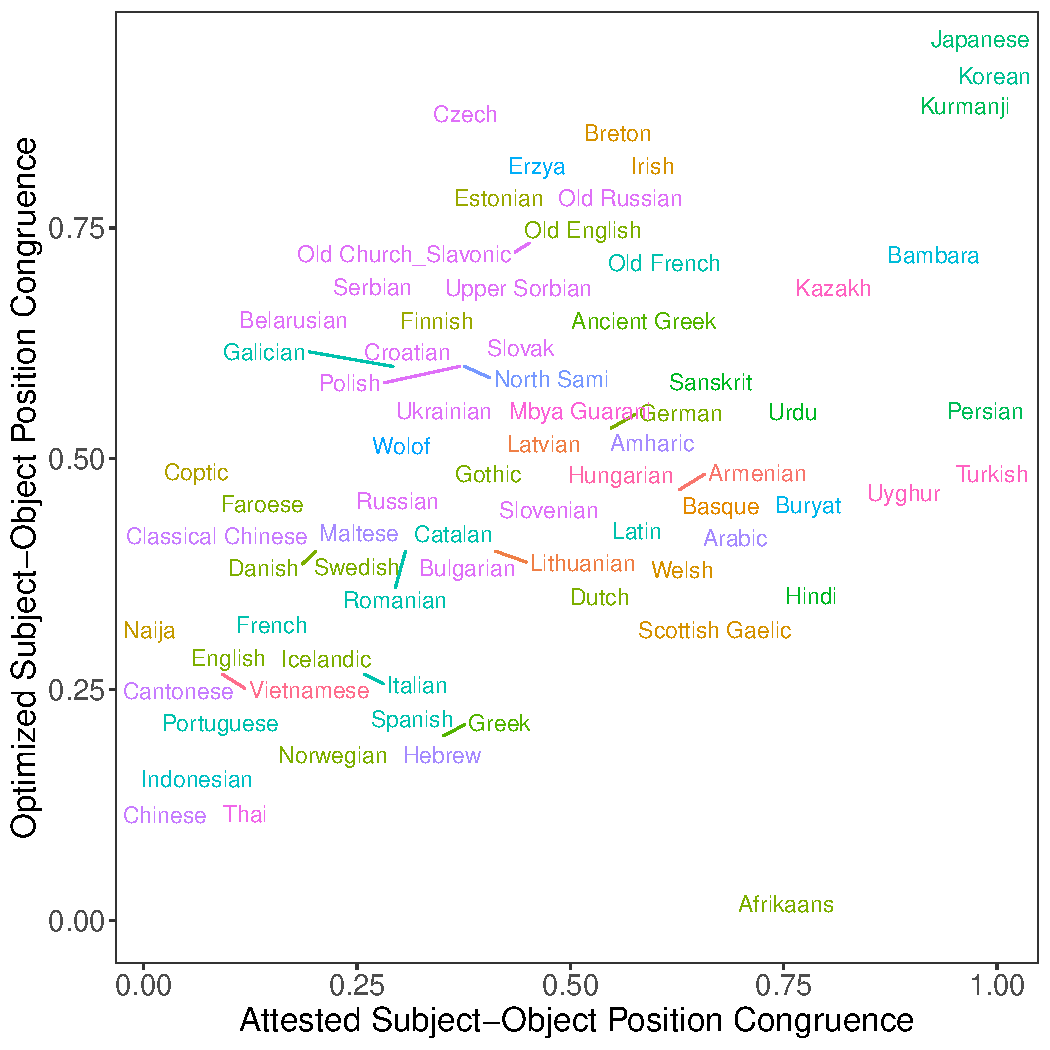
\includegraphics[width=0.4\textwidth]{../analysis/figures/fracion-optimized_DLM_2.6_format.pdf}
    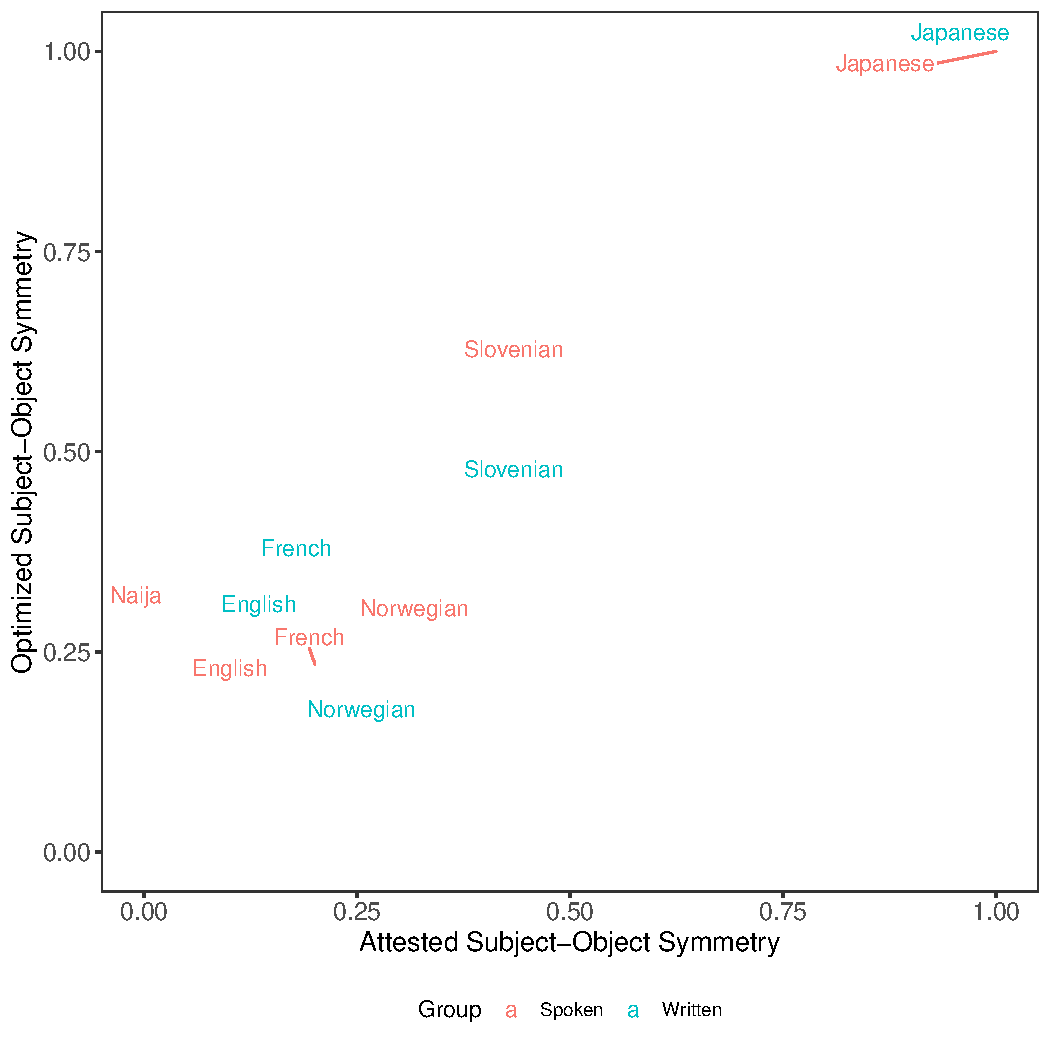
\includegraphics[width=0.4\textwidth]{../analysis/analysis_spoken/spoken.pdf}
    \caption{Left: Subject-object symmetry in attested (x-axis) and approximately optimized (y-axis) orderings. Languages are colored by language families. Small lines connect labels to the position of the language, where needed to avoid overlapping labels. Right: Comparison of subject-object symmetry between written (blue) and spoken (red) corpora in five languages where spoken corpora are available. \mhahn{TODO I'll still think about how to best format these plots.}}
    \label{fig:study1}\label{fig:spoken}
\end{figure}


%\section{Analysis 2: Spoken Corpora}

%\comment{maybe somewhere here or nearby you should acknolwedge that there are only very limited number spoken corpora available, but nevertheless we found these and suggest that these languages span the spectrum of word order variation.}


We have approximated the usage distribution over syntactic configurations using corpora.
However, the vast majority of existing annotated corpus data is in written form (e.g., news and web text), whereas spoken language is thought to be most important for language change, particularly since widespread literacy is very recent.
We collected all spoken corpora in dependency format that we could obtain access to, resulting in data from six languages (see Materials and Methods), and tested whether the conclusion of Analysis 1 continues to hold when using data from these treebanks.
Results on these treebanks, and comparison to written data from the same languages, are shown in Figure~\ref{fig:spoken}.
On these five languages, there is a strong agreenent between written and spoken data.
There is a strong correlation between real and predicted subject-object symmetry in both written ($R=0.96$, $p=0.0023$) and spoken ($R=0.94$, $p=0.0048$) data, in agreement with the Coadaptation Hypothesis.
%In a linear regression with subject-object symmetry among optimized grammars as the dependent variable,  ($\beta=1.11$, $SE=0.29$, $95\%$ CrI $[0.58, 1.69]$).\footnote{The small number of datapoints does not support a mixed-effects analysis. Even with strong priors and more iterations, we encountered small values of Tail Effective Sample Size. However, we found qualitatively similar results when excluding either English or Norwegian, in which case all languages come from different families, and the simple linear model is fully appropriate.}.
%This result is in agreement with that from the full set of corpora.
%\mhahn{TODO the other measure}
%\mhahn{what is the dependent and independent variables in the linear regression? (and perhaps why a Bayes LR as opposed to a plain LR? need to justify a bit more}



%\section{Analysis 2: Historical Evolution}


%We also drew on languages where dependency treebanks with data from different stages of the same language are available (see Materials and Methods for details).

%We also drew on languages where dependency treebanks with data from different stages of the same language are available (see Materials and Methods for details).

%The diagonal in Figure~\ref{fig:study1} describes those points where usage and grammar match perfectly in basic word order, i.e., those points where the real order distribution is identical to the order distribution among optimized grammars, given the distribution over tree topologies.
%Therefore, if the coadaptation hypothesis is true, then languages should stay close to or move towards the diagonal in the plane described by predicted and real subject-object symmetry.

So far, we have provided evidence for the Coadaptation Hypothesis using a cross-sectional synchronic analysis of 74 languages.
If variation in word order reflects coadapation between grammar and usage, we should expect to see coevolution of basic word order and usage as languages evolve over time.
To test this, we conducted a phylogenetic analysis of the evolution of usage and word order.
Phylogenetic analyses have previously been applied to studying the evolution of word order patterns \citep{dunn-evolved-2011, maurits2014tracing}.

A phylogenetic analysis allows us to construct an explicit model of language change, drawing on two sources of information:
First, in several cases, our dataset includes data from different stages of the same language (such as Ancient Greek and Modern Greek).
Such datasets provide direct evidence of diachronic development.
Second, using phylogenetic information, the model can also draw strength from purely synchronic data:
Data from related languages may permit inferences about their (undocumented) common ancestor, and thus about possible trajectories of historical change \citep{pagel2004bayesian, dunn-evolved-2011, maurits2014tracing}.


We used a model of random walks on phylogenetic trees \citep{felsenstein1973maximum,pagel1997inferring, pagel2004bayesian} to model how grammar and usage of a language evolve over time, in order to test the Coadaptation Hypothesis.
We describe the state of a language $L$ at time $t$ as a vector $\xi_{L,t} = (X_{L,t}, Y_{L,t})$ in the plane spanned by usage (optimal subject-object symmetry) and grammar (real subject-object symmetry).
Whenever a language splits into daughter languages, the point $\xi_{L,t}$ continues to evolve independently in each daughter language.
As the components of $\xi_{L,t}$ are continuous, we model their change over time using a random walk given by an Ornstein-Uhlenbeck process (\citep{blackwell2003bayesian}, see Materials and Methods for details).
This process is parameterized by rates of change in the two dimensions and the correlation between the changes in both dimensions \citep{felsenstein1973maximum,freckleton2012fast}.
Under the Coadaptation Hypothesis, changes in both dimensions should be positively correlated.
Under the null hypothesis, no such correlation should be expected.
Besides rates of change, the model also incorporates the possibility of a bias towards specific regions of parameter space (e.g., low or high subject-object symmetry).

We obtained phylogenetic trees for the 74 languages in our sample (see Materials and Methods), and inserted historical stages as inner nodes in these trees.
We fitted the parameters of the model using Hamiltonian Monte Carlo methods (see Materials and Methods for details).


%First, for several languages, corpus data from different stages is available.
%For example, there are dependency treebanks both of contemporary English and Old English (approx. 900 AD).
%There are also cases where data is available from the ancestor of several contemporary languages (e.g., Latin is the ancestor of seven languages in our dataset).


%We obtained phylogenferenvnetic trees for the languages in our dataset (see Materials and Methods for details).
%We modified these trees by adding historical stages of existing languages for which we have corpora, such as Old English (approx. 900 AD) as an ancestor of English.



We visualize the results fit in Figure~\ref{fig:drift-model}.
The blue distribution indicates the stationary distribution of the process, i.e., after long-term evolution, a language will tend to be lie within this distribution.
For illustration, we also illustrate predicted direction of future changes in four languages in red (English, Russian, Arabic, Japanese).

According to the model, changes in grammar and usage are positively correlated:
This is reflected both in the short-term directions of change, which concentrate along the diagonal direction, and in the stationary distribution, according to which languages come to concentrate around the diagonal: In the stationary distribution, positions along the two diagonals are strongly correlated ($R=0.73$, $95\%\ CrI\ [0.28, 0.96]$, $Pr(R<0) = 0.0025$).
Model fit was considerably worse in a lesioned model where the correlation between changes in both direction was constrained to be zero (estimated Bayes Factor: 232).


\begin{figure}
    \centering
    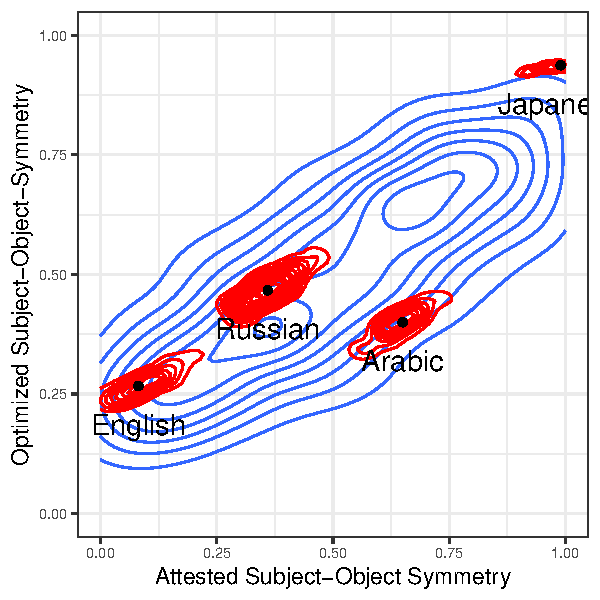
\includegraphics[width=0.5\textwidth]{../change/visualize/stationary.pdf}
    \caption{Result of the phylogenetic drift analysis.
    The blue distribution indicates the estimated long-term stationary distribution of languages, indicating where languages tend to lie after long-term evolution.
    The red distributions indicate predicted states for four individual languages over the next 100 years. Languages are predicted to show co-evolution along grammar (x-axis)  and usage (y-axis). \mhahn{change axis labels}}
    \label{fig:drift-model}
\end{figure}

%\begin{figure}
%    \centering
%    \includegraphics[width=0.5\textwidth]{TODO}
%    \caption{The phylogenetic tree used in our analysis.}
%    \label{fig:phylogenetic-tree}
%\end{figure}


We visualize the evolution of languages where multiple historical stages are documented in Figure~\ref{fig:historical}.
The sample includes multiple languages that started with flexible order and moved towards SVO (English, Romance, East Slavic and Eastern South Slavic, Greek), languages that have remained SVO (Chinese), and languages that have remained predominantly SOV (Indo-Aryan).

In the case of the languages that have remained SVO (Chinese), predicted subject-object symmetry moved towards its true values; that is, these languages appear to have evolved their usage patterns in a way that makes their basic word order more efficient.
The two Indo-Aryan languages in our sample, which have remained predominantly SOV, show little movement in either dimension, slightly away from the diagonal.
Finally, among the remaining languages, which started with flexible order and moved towards SVO, all moved along or towards the diagonal.

%\mhahn{is there a way to also quantify this result?}
%\comment{** yes it might be desirable and even necessary to quantify these results -- is there any alignment metric we can use to determine how well the historical shift aligns with the diagonal, or S-O symmetry reference points? and then compare that alignment metric to some chance value, e.g. by shuffling data across time or era---use this as a null distribution; then report the p-value of the observed, non-shuffled cases? you can then juxtapose the null trajectories (mean + confidence band, in very light color) on the plot to show people how the real trajectory of historical change deviates from the null.}

%We compare to counterfactual trajectories where
%- languages changed only in usage or in order
%- we 

Note that, while our sample includes historical languages that later shifted towards SVO (low subject-object symmetry), it does not include historical languages that later shifted towards SOV (high subject-object symmetry).
The model (and the coadaptation hypothesis) predicts that a language that changed from SVO towards SOV should have correspondingly moved towards the top-right of the plane. 
Currently, no annotated treebanks are available for such a language to directly test this prediction; our prediction can be tested once such a treebank becomes available.
We note that our model indicates no evidence that languages tend to drift towards either SOV or SVO in the long run.
This is shown by the fact that the long-term stationary distribution is equally spread across both low and high subject-object symmetries.
A lesioned version of our model that explicitly prohibits a bias in development provided essentially identical model fit (estimated Bayes Factor 1.1).

A well-known variable covarying with word order is case marking: Languages with case marking are more likely to have free word order, and loss of case marking has been argued to correlate with word order becoming more fixed (CITE) or shifting towards SVO (CITE).
This has a clear functional motivation, because case marking can distinguish subjects and objects when order does not.
In our sample of historical trajectories, movement towards low subject-object symmetry coincides with the loss of case marking in some cases (English, most of Romance, East South Slavic), whereas other languages changed while preserving their case marking systems (Greek and East Slavic).
This raises the question whether our results can be explained away by assuming that both grammar and usage change in response to changes in case marking.
We found that the model continued to predict co-evolution between usage and word order even when controlling for the presence or absence of case, with essentially no change in the predicted strength of correlation (see SI Section XX).
This shows that languages show coadaptation between word order and usage patterns beyond what is captured by the presence of absence of case marking.

%The model provides no evidence that language evolution favors high or low subject-object %asymmetry.
%Visually, the stationary distribution in Figure~\ref{fig:drift-model} is essentially centered with equal weight given to low and high real subject-object symmetry.
%a lesioned model explicitly enforcing absence of such a bias provided essentially identical model fit (Bayes Factor TODO).
%While this conclusion is based on our sample of 74 languages for which dependency treebanks are available, it agrees with the results of \citep{maurits2014tracing} based on a larger sample of languages (albeit from a smaller number of families).

\begin{figure}
    \centering
    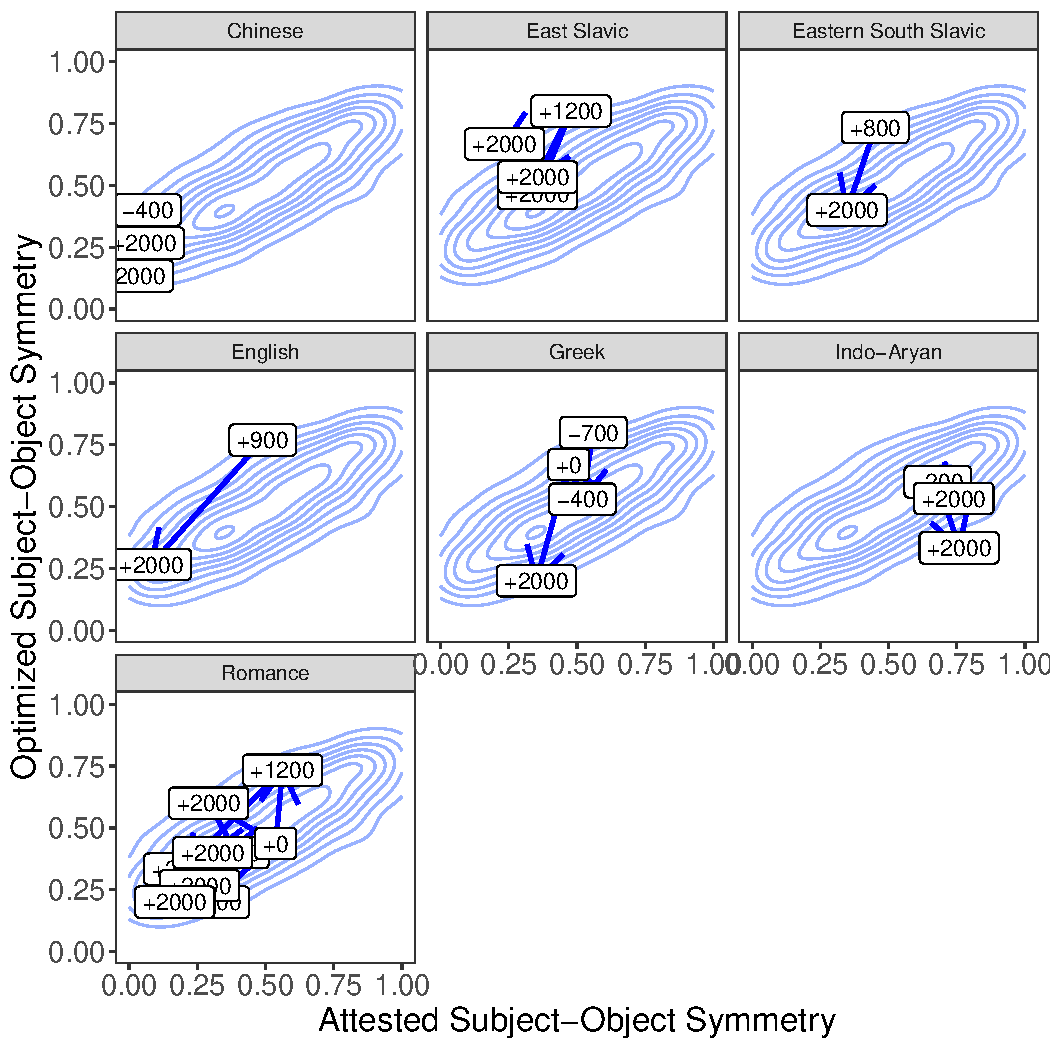
\includegraphics[width=0.95\textwidth]{../analysis/figures/historical_2.6_times_stationary.pdf}
    \caption{The evolutionary trajectories of change in seven languages or language families with documented ancestors. For each point in the trajectories, we indicate an approximate date. The blue background distribution indicates the long-term stationary distribution of all languages combined according to the phylogenetic analysis. \mhahn{change axis labels}}
    \label{fig:historical}
\end{figure}




%\section{Analysis 3: Co-Expression of Subjects and Objects}

%\mhahn{TODO I'll still expand this section}
%\comment{description here seems a bit brief; elaborate more? or say in what way is this result interesting, or surprising, or novel (to the literature)?}



\begin{figure}
    \centering
    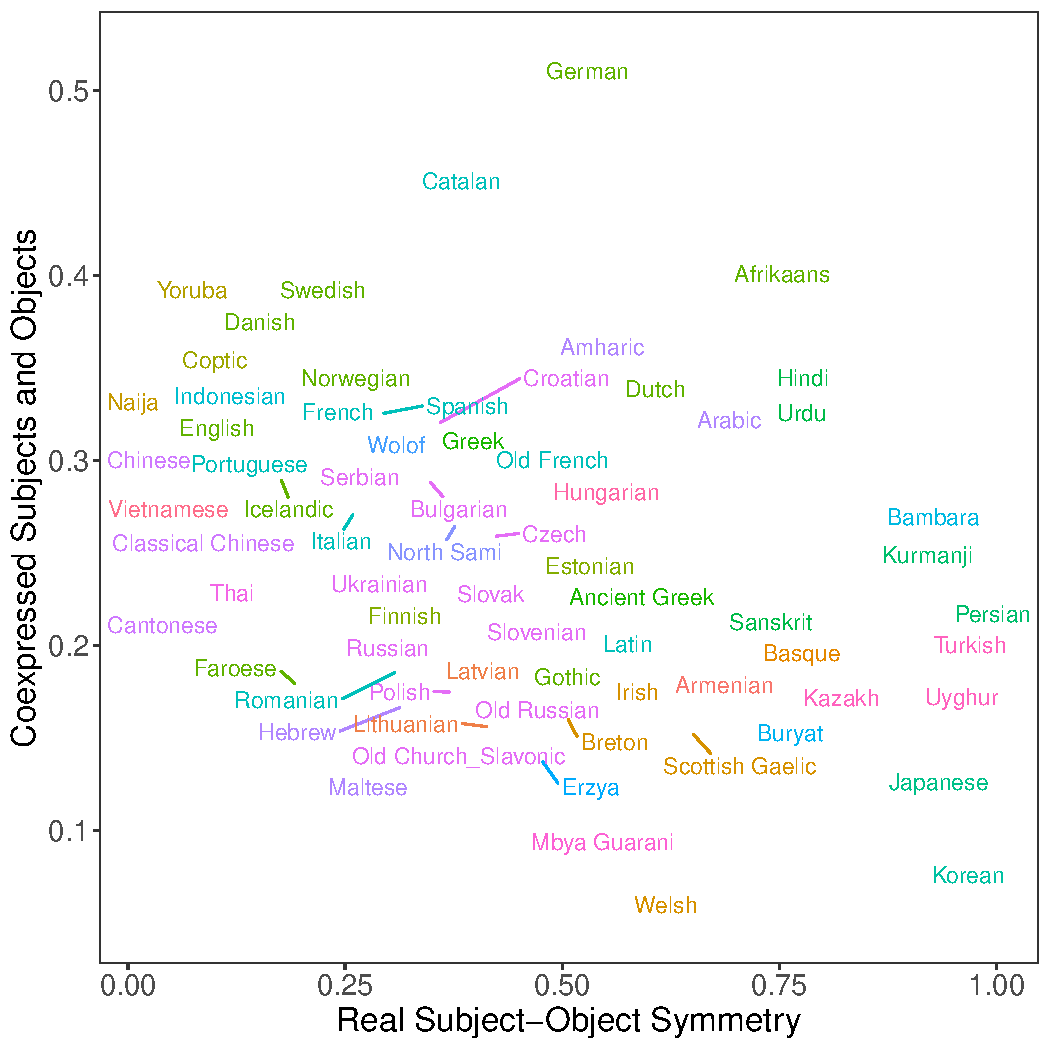
\includegraphics[width=0.7\textwidth]{../analysis/figures/objects-order-pureud-byVerb_FORMAT.pdf}
    \caption{Study 2 (Coexpression of suibjects and objects)}
    \label{fig:study2}
\end{figure}

So far, our results provide evidence for coadaptation between usage and basic word order in the evolution of language.
In what aspects of usage patterns do languages differ and change to realize this coadaptation?
That is, in what ways do usage patterns influence which basic word order is optimally efficient?
Based on the discussion in the introduction, we hypothesized that languages favor SOV-like orders more when they do not frequently coexpress subjects and objects on a single verb.
We quantified the frequency of co-expression of subjects and objects by calculating what fraction of all verbs that realize at least a subject or an object simultaneously realize both.
We show this ratio together with attested subject-object symmetry in Figure~\ref{fig:study2}.
In a linear mixed-effects models, with by-family intercept and slope, observed subject-object symmetry was predictive of this fraction ($\beta=-0.11$, $SE=0.05$, $95\%$ CrI $[-0.21, -0.01]$).
Optimized subject-object symmetry was also predictive of this fraction ($\beta=-0.13$, $SE=0.06$, $95\%$ CrI $[-0.24,  -0.02]$).
These results were not accounted for by differences in the availability of pro-drop (see SI Section X).
We also find evidence for a relation between order and co-expression within individual languages (see SI Section X). %In many languages, subjects of intransitive verbs -- verbs which do not take an object -- can sometimes appear after the verb (e.g., ``along came a dog'', see SI Section X).
%This provides evidence that, when languages show variation between different word order patterns, the choice of word order for a sentence helps optimize for DLM.
%Within languages, we found that individual sentences tend to have the basic word order that optimizes DLM (see SI Section XX).




%We do not find evidence between order and the frequency of embedding on the between-language level (TODO), but there is evidence within languages.
%In some predominant VSO languages, SVO is an alternative word order in unembedded clauses (e.g., Standard Arabic, Berber, Ancient Egyptian, see SI Section X).
%Conversely, in some SVO languages, embedded clauses may show VSO order (Bantu, see SI Section X).




%Say something specific:
%Furthermore, we specifically considered what distinguishes the tree topologies of Old English from those of Modern English.
%- Old English -- English what distinguishes the tree structures?
%In this respect, Old English patterned more like contemporary Japanese.




%- Continental West Germanic (except Yiddish). Main clauses predominant SVO/OSV; embedded clauses SOV/OSV.
%- languages with predominant VSO, but alternative SVO in matrix clauses: Standard Arabic, Berber, Ancient Egyptian
%- relative clauses in Bantu: Demuth,Katherine,andCarolynHarford.1999.Verb raising and subject inversion in Bantu relatives. Journal of African Languages and Lingustics20:41ñ61.


%\section{Discussion}


%{\color{blue} 1. how this work impacts the research on basic word order, and particularly, extends the theory of efficient communication and suggests new functional pressures in shaping the evolution of syntactic structure.}\\

%{\color{blue} 2. how this work is limited.}

\section*{Discussion}

We have investigated the question of what explains the distribution of word order patterns across languages.
We have argued that the observed crosslinguistic distribution of basic word order can be explained as resulting from coadaptation between grammar and usage.

Our work combines evidence from richly annotated syntactic corpora with phylogenetic modeling. We believe that this modeling approach can be useful more generally for studying the fine-grained evolution of grammar.

The theory of coadaptation does not privilege either grammar or usage as being the primary causal driver.
Instead, any language includes both grammar and usage, and they evolve together.
While, in a given language, a change might first appear in one domain, the preservation of efficiency can lead to compensating changes in the other domain.
Consequently, grammar and usage constrain each other in their evolution.

Variation between the grammars of different languages, and change of languages over time, pose an interesting question for existing efficiency-based explanations.
In existing effucuency-based models, differences between languages have been interpreted as reflecting different optima or points along a Pareto frontier \citep{zaslavsky2018efficient, hahn2020universals}.
Language evolution over time can be interpreted as movement along a Pareto frontier of optimal points \citep{zaslavsky2019evolution}.
%As mentioned above, there is evidence that differences in culture may determine differences in vocabulary \cite{gibson2017color}.
The theory of coadaptation adds a new interpretation of differences between languages, by highlighting that individual aspects do not evolve towards efficiency in isolation; rather, we argue that language as a whole evolves to maintain efficiency.
Under this view, cross-linguistic variation in one area, such as basic word order, may be accompanied by variation in another area, such as usage distributions, resulting in an overall efficiency optimization.


%suggest that color naming systems are efficient given the usefulness of color in a society.

%\paragraph{More detailed discussion of previous work (should partly go into intro?}
%There are a range of previous theories of basic word order variation.


%(Gell-Mann  &  Ruhlen,  2011;  Givón,  1979;  Newmeyer,  2000a,  2000b).
% (Senghas,  Coppola,  Newport,  &  Supalla,  1997
% Sandler, Meir, Padden, & Aronoff, 2005
% Goldin-Meadow, So, Ozyurek, and Mylander (2008) 
% (Goldin-Meadow  et  al.,  2008), and Italian (Langus & Nespor, 2010)
%Gershkoff-Stowe L, Goldin-Medow S (2002) Is there a natural order for expressingsemantic relations?Cognit Psychol45(3):375–412.13. 
%Sandler W, Meir I, Padden C, Aronoff M (2005) The emergence of grammar: Sys-tematic structure in a new language.Proc Natl Acad Sci USA102(7):2661–2665.14. 
%Goldin-Meadow S, So WC, Ozyürek A, Mylander C (2008) The natural order of events:How speakers of different languages represent events nonverbally.Proc Natl Acad SciUSA105(27):9163–9168.15. %Langus A, Nespor M (2010) Cognitive systems struggling for word order.CognitPsychol60(4):291–318
%\cite{gibson-noisy-channel-2013} argue that SVO order is more robust under noise in communication for semantically reversible events, because deletion of one argument due to noise makes meaning recovery easier when arguments are on different sides of the verb.
%Under this account, the high prevalence of SOV order is explained by the idea that SOV is the more default order, and that SVO order later results from shift.
%Indeed, there is evidence that SOV emerges spontaneously in gestural communication (CITE).
%\cite{maurits2014tracing} apply phylogenetic modeling to infer how frequently different changes in basic word order are.
%They do not find evidence that one of SOV or SVO is favored over the other in language change, and that languages can cycle between these two orders over time.
%They do, however, find evidence that ancestral languages of multiple families were SOV.

%\cite{ferrer-i-cancho-placement-2017} argues that the variation is caused by a tension between optimizing DLM (thought to favor SVO) and making the verb predictable (thought to favor SOV). This hypothesis is predicated on the idea that DLM favors SVO, which our empirical results will show is not true in general.


%\section{Conclusion}

\section*{Methods}

%{\color{blue}Detailed methods for reproducing this work are typically written in the last section in a NHB article. Include data and code repo and explicit statement that will support replicating all the findings.}\\

%{\color{blue}Prepare supplementary material if need be, e.g., you might want to insert a table and map of all languages and their families, dates or periods of time covered, and their word order(s) etc, as well as the detailed experimental parameters.}



\paragraph{Ordering Grammars}

The counterfactual order grammars have a weight in $[-1, 1]$ for every syntactic relation annotated in the corpora (e.g., subject, object).
Dependents of a head are ordered around it in order of these weights; dependents with negative weights are placed to the left of the head, others to its right.
Optimized grammars are created using the gradient descent method described by \citep{hahn2020universals}.

%Unlike most real languages, these grammars do not model word order freedom; accounting for it 
%- flexible

%$a = \sum_i a_{x_i}$

%where $x$ is a feature vector encoding relevant properties of the word. Concretely, we choose the following:
%- dependency label and POS tag
%- dependency label and POS tag and length of the constituent
%- for each sibling, its dependency label + POS tag + length of the constituent

%While (CITE) introduced this stochastic parameterization to enable gradient-based optimization, we use it to model word order flexibility.

%\paragraph{Creating Optimized Grammars}



\paragraph{Data}
We primarily drew on the Universal Dependencies 2.6 treebanks, we included every language for which a training set with at least 500 sentences was available.
In addition the data available in Universal Dependencies 2.6, we added an Old English dependency treebank in a slightly different but comparable version of dependency grammar (CITE).
While there are some other historical treebanks such as the Penn Parsed Corpora of Historical English (CITE) they are not in the dependency format; calculating dependency length is highly nontrivial without a high-quality conversion.

As the Ancient Greek data available in Universal Dependencies spans multiple stages of the language, we split it in three conventional stages (Archaic 700--500 BC, Classical 500--300BC, and Koine 300BC--300AD, \citet{taylor1994change}) for the phylogenetic analysis. 
%We excluded medieval Latin data as it does not reflect a living language.

We obtained spoken treebanks from the following sources.
For four languages, there are spoken treebanks in the UD project (Slovenian, Naija, Norwegian, French). For Japanese, we used Tueba J/S, a treebank of telephone conversations (CITE). For English, we used an automated conversion (CITE) of the Switchboard section of the Penn Treebank (CITE) to Universal Dependencies.

We obtained the topology of phylogenetic trees from Glottolog (CITE), inserted documented historical languages as inner nodes, and assigned dates for the other inner nodes based on the literature (see SI Section X for details).

\paragraph{Model of Language Change}

% Bayesian inference for Markov processes with diffusion and discrete components
% https://onlinelibrary-wiley-com.stanford.idm.oclc.org/doi/full/10.1111/biom.13292 Latent Ornstein‐Uhlenbeck models for Bayesian analysis of multivariate longitudinal categorical responses
%- Brownian motion (Phylogenetic Independent Contrasts): Model the direction of change. 

%\begin{equation}
%    dX_t = A dB_t
%\end{equation}

We model the state of the grammar of a language $L$ as $X_L$, the observed subject-object symmetry.
As the data for optimized grammars comes in the form of counts (each optimized grammar has subject-object symmetry of $0$ or $1$), we model the usage of a language $L$ as a latent variable $Y_L$ that defines the log-odds that an optimized grammar has a subject-object symmetry of 1 (as opposed to 0).
$X_L$ and $Y_L$ together form the state $\xi_L \in \mathbb{R}^2$  of the language.

%In its simplest form, the model can be described informally by the following update equations, describing how $\xi$ changes over a time interval of length $\Delta$:
%\begin{align}
%    X_{t+\Delta} &= X_{t} + \epsilon_1 \\
%    Y_{t+\Delta} &= Y_{t} + \epsilon_2 \\
%\end{align}
%where $\epsilon_1, \epsilon_2$ are random changes that are modeled as draws from Gaussians.
%Under the coadaptation hypothesis, change in both directions is positively correlated: $Cor(\epsilon_1, \epsilon_2) > 0$.
%Under the null hypothesis, there is no such correlation.
%See Materials and Methods for a rigorous specification of this model.


A common choice in phylogenetic modeling of coevolving traits is correlated Brownian motion, also known as the Independent Contrasts model \citep{felsenstein1973maximum,freckleton2012fast}.
We found that substantially better model fit was achieved by adding a drift term that prevents unbounded values  in long-term evolution (see SI Section X for comparison).
This leads to an Ornstein-Uhlenbeck process \citep{blackwell2003bayesian}, described by the following stochastic differential equation for the instantaneous change of the state $\xi_{L,t}$ of a language $L$ at a given time $t$:
\begin{equation*}
    \operatorname{d}\xi_{L,t} = \Gamma \cdot (\xi_{L,t}-\mu) \operatorname{d}t + \Lambda \operatorname{d}B_t
\end{equation*}
where $\mu \in \mathbb{R}^2$,  $\Gamma, \Lambda \in \mathbb{R}^{2\times 2}$ are non-degenerate matrices, $\Gamma$ is diagonal with positive entries, and $B_t$ is Brownian motion in two dimensions.

The dynamics of stochastic change are described by the second term, $\Lambda \operatorname{d}B_t$:
The diagonal entries of $\Lambda$ encode rates of change in the two dimensions; the off-diagonal encodes correlation \citep{felsenstein1973maximum,freckleton2012fast}: Positive entries in the off-diagonal mean that languages drift in such a way that $X_L, Y_L$ are positively correlated; zero off-diagonal entries indicate independent change in both dimensions.



The other term, $\Gamma \cdot (\xi_{L,t}-\mu) \operatorname{d}t$, encodes deterministic drift, and describes which region $\mu \in \mathbb{R}^2$ of parameter space languages tend to concentrate around in the long run.
The term encodes the fact that the possible range of $\xi_{L,t}$ is bounded and allows the model to encode the possibility of a bias towards some region of the plane.
Without this first term (i.e., with $\Gamma =0$), the simpler Independent Contrasts model \citep{felsenstein1973maximum,freckleton2012fast} would result. See SI Section XX for results from that simpler model and model comparison.

Lesioned models referenced in the text are obtained by setting the off-diagonals of $\Lambda$ to zero (no correlations between change in two dimensions), and $\mu_1=0.5$ (no bias towards high or low real subject-object symmetry).
See SI Section X for additional models that take areal convergence into account.
%In each language family, we modeled the state $\xi_{L,t}$ of the root (e.g., Proto-Indo-European) as a draw from the stationary distribution.

We conducted Bayesian inference using Hamiltonian Monte Carlo in Stan \citep{homan2014the,carpenter2017stan} and computed Bayes factors using Stepping Stone Sampling \citep{xie2011improving}.
See SI Section X for implementation details.




\bibliography{literature}
\bibliographystyle{natbib}

\appendix

\section{Historical Languages}


Dating attested historical languages:

\begin{tabular}{llp{10cm}llll}
Language & Time & Rationale \\ \hline
Coptic & 400 AD & Dating of the Apophthegmata Patrum texts used in the UD treebank\\
Gothic & 350 AD & Life of bible translator Ulfilas (311--383)\\
Old Russian & 1200 AD & Approximate mean age of texts used\\
Old French & 1200 AD  & Approximate mean age of texts used\\
Old English & 900 AD & Approximate mean age of texts used \\
Sanskrit & 200BC & Approximate mean age of texts used \\
Classical Chinese & 300 BC & Life of Mengzi (died around 300 BC), whose work the treebank is based on \\
Latin & 0 AD & Approximate mean age of texts used \\
Archaic Greek & 700 BC & Approximate mean age of texts used \\
Classical Greek & 400 BC & Approximate mean age of texts used \\
Koine Greek & 0 AD  & Approximate mean age of texts used\\
Old Church Slavonic & 850 AD &  Bible translation after invention of Glagolitic alphabet around 850 AD. \\
\end{tabular}

Here, we describe the languages in Figure (TODO).

\begin{tabular}{llll} \hline
Family & Languages & Dates \\ \hline\hline
Chinese & Classical Chinese & -400  \\
& Cantonese & +2000\\ 
& Mandarin & +2000 \\ \hline
East Slavic & Old Russian & +1200 \\
& Russian & +2000 \\ \hline
English & Old English & +900 \\
& English  & +2000\\ \hline
Romance & Latin &+0  \\
& Old French &+1200\\
& French  & +2000\\
& Italian & +2000\\
& Spanish & +2000\\
& Catalan & +2000\\
& Galician & +2000\\
& Portuguese & +2000\\
& Romanian & +2000\\ \hline
Greek & Archaic Greek & -700 \\
      & Classical Greek & -400 \\
      & Koine Greek & +0\\
& Greek  & +2000\\ \hline
Indo-Aryan & Sanskrit & -200 \\
& Hindi  & +2000\\
& Urdu  & +2000\\ \hline
Eastern South Slavic & Old Church Slavonic & +800 \\
& Bulgarian  & +2000\\ \hline
\end{tabular}

\section{Phylogenetic Tree}

\subsection{Tree Topology}

We obtained tree topologies from Glottolog (CITE).
We only retained interior nodes when more than one of their daughter nodes had languages occurring in our dataset.
The resulting tree topology is displayed in Figure~\ref{fig:tree}.\footnote{Tree obtained with https://icytree.org/.}


\begin{figure}
    \centering
	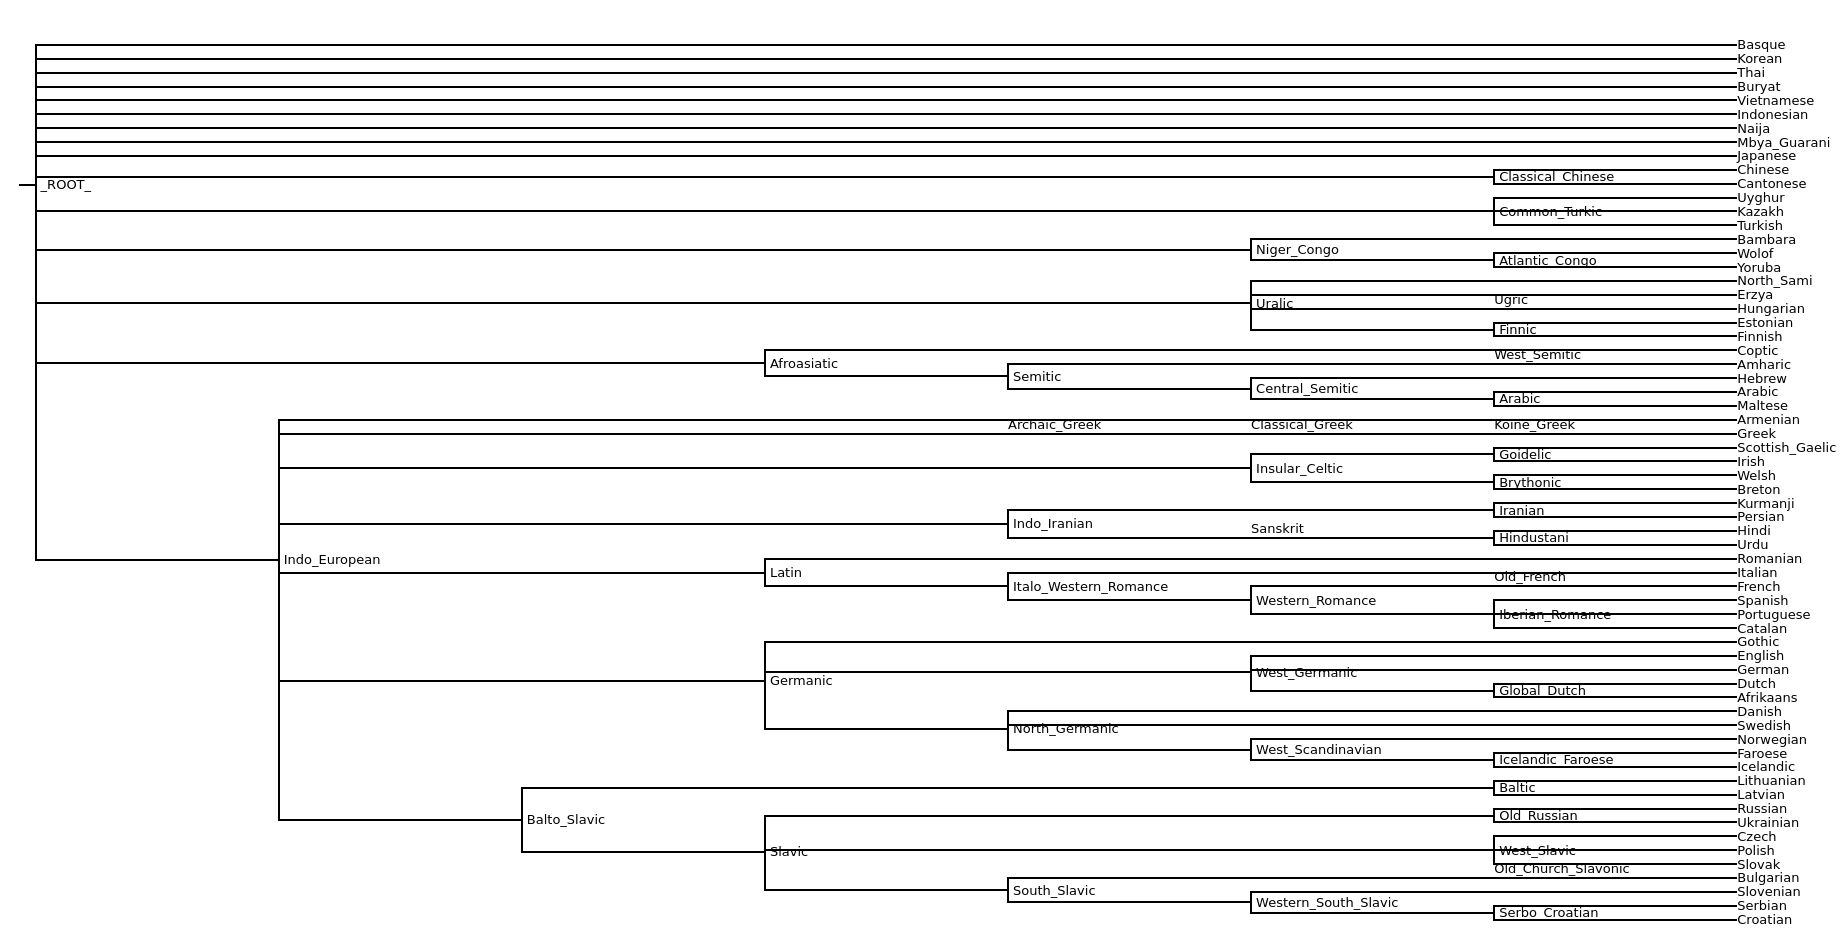
\includegraphics[width=0.9\textwidth]{../trees/tree.png}
       \caption{Phylogenetic tree of the languages in our sample.}
    \label{fig:tree}
\end{figure}




\subsection{Dating Inner Nodes}
We labeled interior nodes for time using estimates based on historical evidence and the linguistic literature.


Dates of split are not always strictly meaningful (e.g. for Romance).



\begin{longtable}{llp{10cm}lll}
Group & Split & Source or Rationale \\ \hline
Afroasiatic & 10,000 BC & \cite{diakonoff1998the} \\
Indo-European & 5,300 BC & \citep{gray2003language} (excluding Hittite and Tocharian, for which we not do not have data). \\
Semitic & 3,750 BC & \citep{kitchen2009bayesian} \\
Insular Celtic & 900BC & \citep{gray2003language} estimate 900BC. Sound shift k$^w$ $>$ p in the Brythonic branch antedates attestation of name `Britain' in 325BC. \\ % Gray and Atkinson: 900BC. Language-tree divergence times support.. Rexova et al, Cladistic analysis
Common Turkic & 700AD & \cite[p. 49]{savelyev2020bayesian} estimate Common Turkic to have split around 474 AD. However, in their model, Old Turkic split off around 650 AD, earlier than the languages in our dataset, with uncertainty about the time of split of the remaining Common Turkic languages. It should predate the earliest documentation of Karluk Middle Turkic after 900AD. We thus put the divergence of the other Common Turkic languages at 700AD. \\
Balto-Slavic & 1,400 BC & \citep{gray2003language} \\
Slavic       & 700AD & \citep{gray2003language}. \citet[p. 209]{novotna2011glottochronology} date the split of East Slavic to the 6th century, \citep{holman2011automated} calibrates it to 550AD. \\
Indo-Iranian & 2,500 BC & \citep[p. 138]{parpola2013formation} \\ % Parpola 1999 suggests 2000 BC. The formation of the Aryan branch of Indo-European.
	Atlantic-Congo & 4,500 BC & \citet{holman2011automated} estimate an age of 6525 years.\\
	Niger-Congo & 5000BC & \citet{holman2011automated} estimate an age of 6227 years, but the family has to be older than Atlantic-Congo. We place Niger-Congo at 5000BC.\\
Uralic & 3,000 BC & \citep[Section 4.7]{maurits2020best}, cf \citep[p. 144]{parpola2013formation} for references \\
Finnic & 800 AD & \cite[Section 4.1]{maurits2020best} \\
West-Semitic & 3,400 BC & \citep{kitchen2009bayesian}  \\
Central-Semitic & 2,450 BC & \citep{kitchen2009bayesian}   \\
South-Slavic & 750 BC & Expansion of Slavic into Balkan. Postdates Slavic and antedates Old Church Slavonic (attested after 800AD) \\
West-Slavic & 750 BC & Expansion of Slavic. \\ %\citet{holman2011automated} calibrates the split between Czech and Slovak at 1050AD.  \\ % , citing Fodor (1962:132),
Iranian & 500 BC & \citep{gray2003language}. (Parpola 1999:200) suggests 1900BC based on archaeological evidence. \\ % Kurmanji, Persian. Parpola 1999 suggests 1900 BC.
Eastern Baltic & 600 AD & Split between Katvian and Lithuanian \citep[p. 209]{novotna2011glottochronology}\\
%Ugric & 2,000 BC & \citep{maurits2020best} \\
Hindustani & 1,800 AD & Standardization of Hindi and Urdu\\
Serbo-Croatian & 1,900 AD & Standardization of Serbian and Croatian\\
Germanic & 250AD & \cite{gray2003language} \\
West-Germanic & 500 AD & Migrations into Britain and southern central Europe\\
North-Germanic & 650 AD & Split of Old Norse into regional variants, such as assimilation of nasals to following stops in Western Norse in the 7th century \citep[p. 1856, 1859]{sandoy2017202}. Similarly \citep{holman2011automated} calibrates this to 900 AD. \\% (e.g. assimilation of nasals to following stop in Western Norse in the 7th century. Bandle 2005, Ch. XVII par. 202, The typological ...I Phonology Old East Nordic, p. 1856, 1859. \\
West-Scandinavian & 1,100 AD & Sound shifts specific to Norwegian\\
Icelandic-Faroese & 1,400 AD & Sound shifts specific to Faroese\\
Goidelic & 950 AD & Migrations from Ireland to Scotland. \citet{holman2011automated}, citing \citet{jackson1951gaelic}, calibrates the divergence between Irish and Scottish Gaelic to 950 AD. \\
Brythonic & 500 AD & Migrations from Britain to Brittany (Humphreys 1993:609. Breton languagem its present position and historical background, cited by holman2011automated)\\
Global Dutch & 1,600 AD & Dutch colony in South Africa \\
Western South Slavic & 1,000 AD & Antedates earliest Slovenian and Serbo-Croatian texts\\
Western Romance & 800 AD & Expansion of Christian kingdoms into Iberia \\
Italo-Western-Romance & 500 AD & End of the Western Roman empire \citep{holman2011automated}.  \\
Iberian Romance & 1,000 AD & Expansion of Christian kingdoms in Iberia, earliest Iberian Romance texts \\
West Iberian & 1,100 & Independence of Portugal \\
Arabic & 1100 AD & Calibration from \citep{holman2011automated} based on end of Arabic domination of Malta.
\end{longtable}


\section{Details for Phylogenetic Models}



%We adopt the model of random walks on phylogenetic trees.
%We model the development of grammar and usage as an Ornstein-Uhlenbeck process (See SI Section X for results with a simpler Brownian motion model).
%According to the model of random walks on phylogenetic trees, whenever a (historical) language branches off into multiple successor languages, they independently develop according to this process.


%As the data for optimized grammars comes in the form of counts, we model the usage of a language $L$ as a latent variable $X_L$ that defines the log-odds that an optimized grammar has a subject-object symmetry of 1 (as opposed to 0).
%We model the state of the grammar as $Y_L$, the observed subject-object symmetry.
%$X_L$ and $Y_L$ together form the state $\xi_L \in \mathbb{R} \times [0,1]$  of the language.

%\subsection{Simple Brownian Motion Model}


%We model the instantaneous change of the state $\xi_t$ a language at a given time $t$ as a correlated Brownian motion in two dimensions:
%\begin{equation*}
%    d\xi_t = \Lambda dB_t
%\end{equation*}
%where $\Lambda \in \mathbb{R}^{2\times 2}$ is non-degenerate.

%\subsection{Model with Drift}

%(See below for likelihood results, showing poor fit of the simple Brownian model).


%\section{Details for Phylogenetic Models}



%We adopt the model of random walks on phylogenetic trees.
%We model the development of grammar and usage as an Ornstein-Uhlenbeck process (See SI Section X for results with a simpler Brownian motion model).
%According to the model of random walks on phylogenetic trees, whenever a (historical) language branches off into multiple successor languages, they independently develop according to this process.


%As the data for optimized grammars comes in the form of counts, we model the usage of a language $L$ as a latent variable $X_L$ that defines the log-odds that an optimized grammar has a subject-object symmetry of 1 (as opposed to 0).
%We model the state of the grammar as $Y_L$, the observed subject-object symmetry.
%$X_L$ and $Y_L$ together form the state $\xi_L \in \mathbb{R} \times [0,1]$  of the language.

%\subsection{Simple Brownian Motion Model}


%We model the instantaneous change of the state $\xi_t$ a language at a given time $t$ as a correlated Brownian motion in two dimensions:
%\begin{equation*}
%    d\xi_t = \Lambda dB_t
%\end{equation*}
%where $\Lambda \in \mathbb{R}^{2\times 2}$ is non-degenerate.

%\subsection{Model with Drift}


%This is expressed by the following stochastic differential equation, known as the Ornstein-Uhlenbeck process:
%We model the instantaneous change of the state $\xi_t$ a language at a given time $t$ as a combination of drift and Brownian motion:
%\begin{equation*}
%    d\xi_t = -A(\xi_t-\mu) + \Lambda dB_t
%\end{equation*}
%where $A, \Lambda \in \mathbb{R}^{2\times 2}$, all eigenvalues of $A$ have positive real part, and $\Lambda$ has full rank.


%The matrix $A$ encodes the direction of drift.
%$A_{1,2}$ encodes the extent to which drift of $X_t$ and $Y_t$ is correlated:
%$A_{1,2} > 0$ means that languages drift in such a way that $X_L, Y_L$ are positively correlated (coadaptation); $A_{0,0} = 0$ means that languages do not drift towards a correlation (See Si Section X for an alternative formulation in terms of correlated Brownian motion).


%We model the instantaneous change of the state $\xi_t \in \mathbb{R}^2$ of a language at a given time $t$ as a combination of drift and Brownian motion, formalized by the following stochastic differential equation defining the Ornstein-Uhlenbeck process \citep[p. 109, eq. 4.4.42]{gardiner1983handbook}:
%\begin{equation*}
%    d\xi_t = -\Gamma \cdot (\xi_t-\mu) dt + \Lambda \cdot dB_t
%\end{equation*}
%where $\mu \in \mathbb{R}^2$, $\Gamma, \Lambda \in \mathbb{R}^{2\times 2}$, the real part of each eigenvalue of $\Gamma$ is positive, and $\Lambda$ has full rank (so that $\Lambda\Lambda^T$ is positive definite).
%is positive definite, and $\Lambda$ is diagonal with positive entries (see SI Section for results with non-diagonal $\Lambda$).


%The matrix $A$ encodes the direction of drift.
%$A_{1,2}$ encodes the extent to which drift of $X_t$ and $Y_t$ is correlated:
%$A_{1,2} > 0$ means that languages drift in such a way that $X_L, Y_L$ are positively correlated (coadaptation); $A_{0,0} = 0$ means that languages do not drift towards a correlation (See Si Section X for an alternative formulation in terms of correlated Brownian motion).


%We model the instantaneous change of the state $\xi_t \in \mathbb{R}^2$ of a language at a given time $t$ as a combination of drift and Brownian motion, formalized by the following stochastic differential equation defining the Ornstein-Uhlenbeck process \citep[p. 109, eq. 4.4.42]{gardiner1983handbook}:
%\begin{equation*}
 %   d\xi_t = -\Gamma \cdot (\xi_t-\mu) dt + \Lambda \cdot dB_t
%\end{equation*}
%where $\mu \in \mathbb{R}^2$, $\Gamma, \Lambda \in \mathbb{R}^{2\times 2}$, the real part of each eigenvalue of $\Gamma$ is positive, and $\Lambda$ has full rank (so that $\Lambda\Lambda^T$ is positive definite).
%is positive definite, and $\Lambda$ is diagonal with positive entries (see SI Section for results with non-diagonal $\Lambda$).


%The matrix $A$ encodes the direction of drift.
%$A_{1,2}$ encodes the extent to which drift of $X_t$ and $Y_t$ is correlated:
%$A_{1,2} > 0$ means that languages drift in such a way that $X_L, Y_L$ are positively correlated (coadaptation); $A_{0,0} = 0$ means that languages do not drift towards a correlation (See Si Section X for an alternative formulation in terms of correlated Brownian motion).

%, for comparison with a simple Brownian motion model, and for comparison with non-diagonal $\Gamma$.
%We adopt the model of Brownian motion on phylogenetic trees.
%As the data for optimized grammars comes in the form of counts, we model the usage of a language $L$ as a latent variable $X_L$ that defines the log-odds that an optimized grammar has a subject-object symmetry of 1 (as opposed to 0).
%We model the state of the grammar as $Y_L$, the observed subject-object symmetry.
%$X_L$ and $Y_L$ together form the state $\xi_L \in \mathbb{R} \times [0,1]$  of the language.
%We model the instantaneous change of the state $\xi_t$ a language at a given time $t$ as Brownian motion:
%\begin{equation*}
%    d\xi_t = \Lambda dB_t
%\end{equation*}
%where $\Lambda \in \mathbb{R}^{2\times 2}$.
%$\Lambda_{1,2}$ encodes the extent to which drift of $X_t$ and $Y_t$ is correlated:
%$A_{1,2} > 0$ means that languages drift in such a way that $X_L, Y_L$ are positively correlated (coadaptation); $A_{0,0} = 0$ means that movement in both directions is not correlated.

%The matrix $\Sigma := \Lambda\Lambda^T$ indicates the variance-covariance structure of the instantaneous changes at any time $t$.
%The main quantity of interest is the correlation between changes in the two dimensions, which is given by
%\begin{equation}
%R := \frac{\Sigma_{1,2}}{\sqrt{\Sigma_{1,1}\Sigma_{2,2}}}
%\end{equation}
%A positive value indicates that changes in both directions are positively correlated.

\subsection{Calculating the Likelihood}
For completeness, we describe how to calculate the likelihood of a multidimensional Ornstein-Uhlenbeck model on phylogenetic trees.

As described in Materials and Methods, it is described by the following stochastic differential equation for the instantaneous change of the state $\xi_{L,t}$ of a language $L$ at a given time $t$:
\begin{equation*}
    \operatorname{d}\xi_{L,t} = \Gamma \cdot (\xi_{L,t}-\mu) \operatorname{d}t + \Lambda \operatorname{d}B_t
\end{equation*}
where $\mu \in \mathbb{R}^2$,  $\Gamma, \Lambda \in \mathbb{R}^{2\times 2}$ are non-degenerate matrices, and $B_t$ is Brownian motion in two dimensions.

In our model, $\Gamma$ is diagonal with positive entries; we found no improved model fit when taking more general choices for $\Gamma$.

The conditional distribution of a future observation at time $t+\Delta$ given an earlier one at time $t$ is given by the following equation \citep[Theorem 3.3]{schach1971weak}, \citep{gardiner1983handbook}, \citep[p. 156, eq. 6.124]{risken1989fokker}:
\begin{equation}
\xi_{L,t+\Delta} | \xi_{L,t} \sim N\left(\mu + e^{-\Delta \Gamma} (\xi_{L,t}-\mu),\ \Omega - e^{-\Delta \Gamma} \Omega e^{-\Delta \Gamma^T}\right)
\end{equation}
where the matrix $\Omega \in \mathbb{R}^{2\times 2}$ is obtained as the solution of the equation \citep[p. 110, eq. 4.4.51]{gardiner1983handbook} \citep[p. 156, eq. 6.126]{risken1989fokker}:
\footnote{Setting $\Sigma := \Lambda\Lambda^T$, this can be solved as follows:
\begin{equation}
\left(\begin{matrix} \Omega_{11} \\ \Omega_{12} \\ \Omega_{22} \end{matrix}\right)=    \left(\begin{matrix}
    2\Gamma_{11} & 2\Gamma_{12} & 0 \\
    \Gamma_{21} & \Gamma_{11}+\Gamma_{22} & \Gamma_{12} \\
    0 & 2\Gamma_{21} & 2\Gamma_{22}
    \end{matrix}\right)^{-1}  \left(\begin{matrix} \Sigma_{11} \\ \Sigma_{12} \\ \Sigma_{22} \end{matrix}\right)
\end{equation}
}
\begin{equation}
    \Gamma\Omega+\Omega\Gamma^T = \Lambda \Lambda^T
\end{equation}
Based on this, one can compute the stationary distribution that solves the differential equation.
The stationary distribution of an individual observation is
\begin{equation}\label{eq:ornuhl-var}
\xi_{t} \sim N\left(\mu, \Omega \right)
\end{equation}
The stationary cross-covariance between the states of two languages $L_1, L_2$, possibly on different branches of the phylogenetic tree, is given by
\begin{equation}\label{eq:ornuhl-covar}
Cov(\xi_{L_1}, \xi_{L_2}) = e^{-\Delta_1 \Gamma} \Omega e^{-\Delta_2 \Gamma^T}
\end{equation}
if $\Delta_1, \Delta_2$ are the times of evolution from their last common ancestor to $L_1$ and $L_2$, respectively.
\footnote{This can be shown as follows:
If $\xi_A$ is the last common ancestor, then (we set $\mu=0$ without loss of generality, as it does not affect the covariance):
\begin{align*}
Cov(\xi_{L_1}, \xi_{L_2}) &= \mathbb{E} \left[\xi_{L_1} \xi_{L_2}^T\right] - \mathbb{E}\xi_{L_1} \mathbb{E}\xi_{L_2}^T   &= \mathbb{E}\left[\mathbb{E} \left[\xi_{L_1} \xi_{L_2}^T | \xi_A\right]\right] - 0 \cdot 0  &= \mathbb{E}\left[\mathbb{E} \left[\xi_{L_1}|\xi_A\right] \mathbb{E} \left[\xi_{L_2}^T | \xi_A\right]\right]  
 &= \mathbb{E}\left[   e^{-\Delta_1\Gamma} \xi_A    \xi_A^T e^{-\Delta_2\Gamma^T} \right]  \\
 &= e^{-\Delta_1\Gamma} \Omega e^{-\Delta_2\Gamma^T}   \\
\end{align*}}
If $L_1, L_2$ do not share a common ancestor (the root in Figure~\ref{fig:tree} does not count as an ancestor), the covariance is zero.\footnote{As $\lim_{\Delta \rightarrow \infty} e^{-\Delta B} = 0$, this is practically equivalent to assuming a very large time-depth of the last common ancestor, which would be the case under the assumption of macrofamilies with very large time depth.}



Since any Ornstein-Uhlenbeck process is Gaussian \citep{schach1971weak}, the joint distribution of any set of observations $\xi_{L, t}$ is determined by (\ref{eq:ornuhl-var}-\ref{eq:ornuhl-covar}).

\subsection{Implementation}

We implemented the models in Stan and obtained posterior samples using the No-U-Turn sampler as implenented in Stan (CITE).
We ran four chains with 2000 iterations each, of which the first 1000 were discarded as warmup samples.

We computed marginal likelihoods using Stepping Stone Sampling (CITE) with $K=10$ stones.
The fact that $Y_L$ is a latent variable complicates computation of the likelihood; we approximated this by fixing $Y_L$ to the log-odds of the observed empirical counts, adding $1$ to each category.
We verified stability of the estimates by running the procedure ten times for each model, and averaging the obtained marginal likelihoods.


\subsection{Quantifying Instantaneous Correlation}
The matrix $\Sigma := \Lambda\Lambda^T$ indicates the variance-covariance structure of the instantaneous changes at any time $t$ \citep{felsenstein1973maximum, freckleton2012fast}.
The main quantity of interest is the correlation between changes in the two dimensions, which is given by
\begin{equation}
R := \frac{\Sigma_{1,2}}{\sqrt{\Sigma_{1,1}\Sigma_{2,2}}}
\end{equation}
A positive value indicates that changes in both directions are positively correlated.

%\paragraph{Computing Likelihood for Brownian Motion Model}

%We impose an LKJ prior on the correlation matrix of $A$, a student $t$ prior on the variance components of $A$ and $\Lambda$, a ... prior on the two components of $\Lambda$.

%\paragraph{Computing Likelihood for Ornstein-Uhlenbeck Model}

\section{Comparison with Simple Brownian Model}

The simple Brownian model leaves out the drift term, leading to the stochastic differential equation:
\begin{equation*}
    \operatorname{d}\xi_t = \Lambda \operatorname{d}B_t
\end{equation*}
This is known as the Independent Contrasts model \citep{felsenstein1973maximum, freckleton2012fast}.

Brownian motion differs from the Ornstein-Uhlenbeck process in that it does not have a long-term stationary solution.
Instead, trajectories $\xi_t$ tend to move arbitrarily far away from the origin over time $t$.
This is clearly unrealistic in our setting, as subject-object symmetry is bounded between 0 and 1.

As there is no stationary solution, there is no straightforward way to jointly apply the model to data from languages that do not share a common ancestor.
For modeling purposes, we assumed that all families had a common ancestor at some large time $T_0$ in the past.
This modeling assumption corresponds to the assumption of macro-families of very large time-depth.
We varied $T_0$ from 10,000 BC to 100,000 BC, and measured the instantaneous correlation of changes $R$ for each fit.
To evaluate model fit, we compared marginal likelihood of the Brownian model with the Ornstein-Uhlenbeck model.

\paragraph{Results}
Across different choices of $T_0$, the Brownian model strongly supports a positive correlation $R$, very similar to the Ornstein-Uhlenbeck analysis.

Model fit as measured by marginal likelihood is considerably weaker in the Brownian model, across choices of $T_0$ (BVayes Factor TODO).

%This limitation can be addressed by adding a drift term, whereby languages tend to stay within a bounded area, while subjected to random walk dynamics within this area.


\section{Accounting for Areal Convergence}
We accounted for effects of geographic neighborhoods by modeling linguistic areas.
We modeled linguistic areas as latent variables defining time- and location-dependent values $\mu(x,t)$ (where $x$ is a point on the surface of the earth and $t$ is a point in time) that languages at time $t$ and place $x$ drift towards.

\paragraph{Model}
We model the grammar and usage components of $\mu$ to depend on the language's geographic position and the time a language was spoken.
This models the impact of linguistic areas, and allows this impact to change over time.

We assume that the development of a language $L$ observed at time $t+\Delta$ (e.g. English) developed from a prior state at time $t$ (e.g., Old English) during time $[t, t+\Delta]$ according to the Ornstein-Uhlenbeck SDE
\begin{equation*}
    \operatorname{d}\xi_{L,t} = \Gamma \cdot (\xi_{L,t}-\mu_L) \operatorname{d}t + \Lambda \operatorname{d}B_t
\end{equation*}
where $\mu_L$ is defined by the temporal and geographical location of the language $L$.


We placed a Gaussian process prior with a Laplace kernel on $\mu$.
That is, the covariance between $\mu$ at points $x, y$ on the surface of the earth at times $T_1, T_2$ was taken to be
\begin{equation}\label{eq:kernel}
    Cov(\mu_x, \mu_y) = \alpha \exp\left(-\frac{1}{\rho^2_1} d(x,y) - \frac{1}{\rho_2^2} |T_1-T_2|\right)
\end{equation}
where $d(x,y)$ is the great circle (geodesic) distance between points $x, y$.
The Laplace kernel is positive-definite with the great-circle distance $d(\cdot, \cdot)$ (CITE), whereas the commonly used RBF kernel is not positive-definite.

We extracted locations of languages from WALS.
For ancestors, we recursivdefined their location as the mean of the locations of their immediate children.

We placed the priors ... on the parameters of the kernel~(\ref{eq:kernel}).

As $\mu$ now varies with time, the resulting process is not Gauss-Markov any more \citep{schach1971weak}, and thus the likelihood cannot be represented with a single covariance matrix any more.
We thus perform inference by explicitly modeling $\xi_L$ for all inner nodes $L$ of the phylogenetic tree.



\paragraph{Results}
We plot the posterior of the correlation component of $\Sigma$ in Figure~\ref{fig:posterior-area-time}.
The posterior probability that the correlation is $\leq 0$ is estimated to be TODO.

%In Table, we show all models together with the logarithm of the estimated marginal likelihood of the data.
%Higher marginal likelihood indicates better model fit.


%Conditions:
%- $\Gamma$ has positive eigenvalues
%- $\Gamma\Omega+\Omega\Gamma^T$ is a covariance matrix
%- $\Omega$ is a covariance matrix
%Things to visualize
%- stationary distribution
%- instantaneous distribution over change directions


% https://courses.helsinki.fi/sites/default/files/course-material/4523939/Freckleton02.pdf


\section{The Role of Case Marking}

Here, we test whether our results can be explained away by assuming that word order and usage patterns independently change in response to the presence or absence of case marking.
We do this by fitting an extension of the model that can model different directions of change in languages with and without case marking, and checking whether the analysis continues to provide evidence for coevolution between word order and usage.

\paragraph{Coding Languages for Case Marking}
We coded languages from our sample for the presence or absence of case marking on the basis of \citep{iggesen2013number}, supplemented with information from the grammatical literature where no information was provided.
We amended the annotation from \citep{iggesen2013number} to include only case marking that distinguishes between subjects and objects; this concerns several modern Celtic and Germanic languages, which have some nominal case marking but do not distinguish subjects and objects (e.g., Swedish and English use -\textit{s} to mark possessives, but do not distinguish nominal subjects and objects.).

We furthermore coded all interior nodes of the phylogenetic tree for case marking based on the linguistic literature.
In some cases, this annotation was unambiguous due to available historical documentation even though no treebank data was availavble (e.g., Proto-West-Scandinavian was a late form of Old Norse and had case markers).
In many other cases, cognate case markers are unambiguously attested both within and without a group, showing that they were present in the protolanguage (e.g., Proto-Germanic, Proto-Indo-Iranian).
Furthermore, in many protolanguages, case markers are commonly reconstructed based on their presence in different descendant branches (e.g., Proto-Indo-European, Proto-Afroasiatic, Proto-Common-Turkic, Proto-Uralic and Proto-Ugric). % Uraloc: Abondolo Uralic; Hajdu uralischen Sprachen; Marcantonio Uralic
Case is not unambiguously reconstructed for Proto-Niger-Congo and Proto-Atlantic-Congo; we verified that all four possible parameter settings lead to equivalent results (we report results under the assumption that neither of them had case, with essentially indistinguishable results for the other cases).

\paragraph{Model of Change conditioned on Case Marking}
Based on the prior literature, we expect that languages without case marking will be biased towards low subject-object symmetry (CITE).
To take this into account, we modified the model by conditioning the mean vector $\mu$ on the presence or absence of case in the language $L$.
\begin{equation*}
    \operatorname{d}\xi_{L,t} = \Gamma_{C(L)} \cdot (\xi_{L,t}-\mu_{C(L)}) \operatorname{d}t + \Lambda \operatorname{d}B_t
\end{equation*}
where $C(L)$ is $1$ if $L$ has case and $0$ else.
We set priors $\mu_{C(L)} \sim N(0,1)$ for both $C(L) = 0$, and $1$.


\paragraph{Results}
We plot the distribution of languages and the fitted stationary distributions, conditioned on $C(L)$, in Figure~\ref{fig:langs-case}.
In accordance with the prior literature, the model indicated that languages without case marking favor regions with low observed and optimized subject-object symmetry (TODO).
For languages with case marking, there was evidence for a bias towards higher subject-object symmetry (TODO).
We plot the posterior of the correlation component of $\Sigma$ in Figure~\ref{fig:posterior-case} (top).
The posterior probability that the correlation is $\leq 0$ is estimated to be $0.0055$.

To separately estimate the evidence coming from languages with or without case marking, we also fitted a model where $\Lambda$ was also dependent on $C(L)$.
The resulting correlation component posteriors are shown in Figure~\ref{fig:posterior-case} (bottom).
We found a positive correlation in both settings individually (posterior of non-positive correlation $0.04175$ with case, $0.0385$ without case).

\paragraph{Conclusion}
We found that case marking has a strong impact on subject-object symmetry, and that coadaptation continues to hold when controlling for this.

\begin{figure}
    \centering
    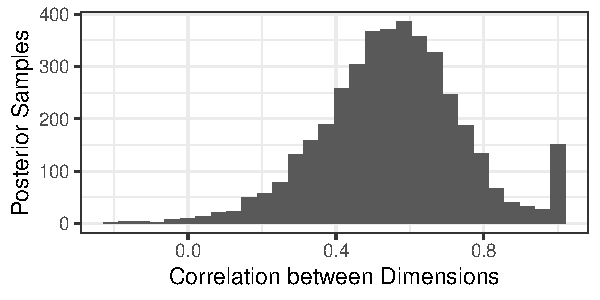
\includegraphics[width=0.3\textwidth]{../change/visualize/figures/corr_ornuhl-binom_42.pdf}
    
    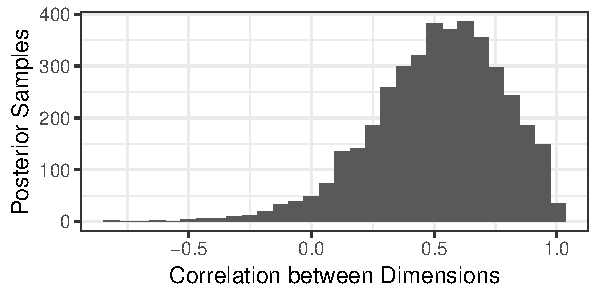
\includegraphics[width=0.3\textwidth]{../change/visualize/figures/corr_ornuhl-binom_45_Case.pdf}
    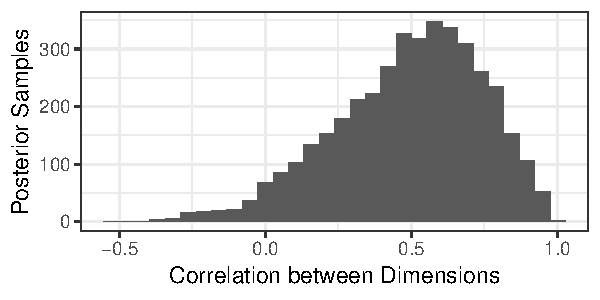
\includegraphics[width=0.3\textwidth]{../change/visualize/figures/corr_ornuhl-binom_45_NoCase.pdf}
    \caption{Posterior of the Usage-Grammar correlation coefficient $R$ when accounting for case marking. Top: Assuming a joint $\Sigma$. Bottom: Assuming separate values for $\Sigma$.}
    \label{fig:posterior-case}
\end{figure}

\begin{figure}
    \centering
    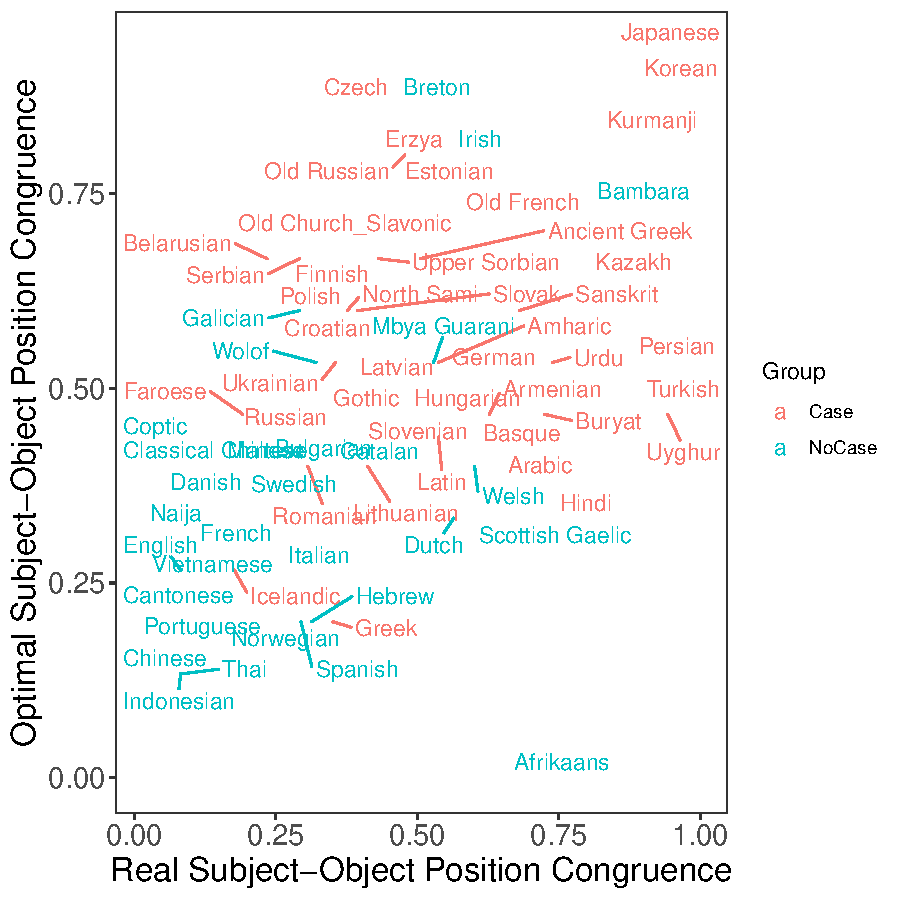
\includegraphics[width=0.4\textwidth]{../analysis/figures/by_patient_marking.pdf}
    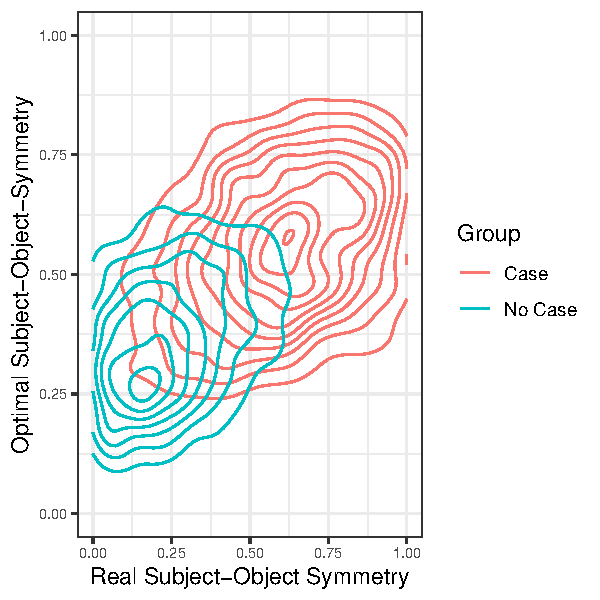
\includegraphics[width=0.4\textwidth]{../change/visualize/stationary_case.pdf}
    \caption{Left: Languages by availability of morphological distinction between subject and object nouns. Right: Fitted stationary distribution, conditioned on case marking.}
    \label{fig:langs-case}
\end{figure}

%#Oliver A. Iggesen. 2013. Number of Cases.
%#In: Dryer, Matthew S. & Haspelmath, Martin (eds.)
%#The World Atlas of Language Structures Online.
%#Leipzig: Max Planck Institute for Evolutionary Anthropology.
%#(Available online at http://wals.info/chapter/49, Accessed on 2020-09-20.)


%\section{Pro-Drop}
%This correlation was not accounted for by differences in the availability of pro-drop (see SI Section X).


%Say something specific:
%Furthermore, we specifically considered what distinguishes the tree topologies of Old English from those of Modern English.
%- Old English -- English what distinguishes the tree structures?
%In this respect, Old English patterned more like contemporary Japanese.

\section{Within-Language Correlates of Basic Word Order}

Here, we show that basic word order reflects optimization for DLM not only on the level of languages, but also on the level of individual sentences.

\subsection{Coexpression: VS Order in SVO Languages}
In many SVO languages, certain intransitive subjects can appear after the verb (``along came a dog'' CITE).

%- literature
%- Unaccusative inversion
%-- Leonetti, Two Types of postervbal subject (Spanish): Unaccusative inversion (p. 17)
%-- English there inversion

We conjectured that, more generally, the rate of VS order is higher when no object is present than when an object is present.
For each language in our dataset, we collected statistics for all verbs with a subject and conducted the following logistic analysis:

\begin{equation}
\text{SV Order} \sim \text{Object is present}
\end{equation}

A positive effect indicates that presence of an object makes SV order more likely, compared to VS order.
Results are shown below.
As predicted, in most languages where there is variation between SV and VS order, a significant positive effect was observed.

\begin{longtable}{l|lllllll}
Language & SV Frequency & $\beta$ & $p$ \\ \hline
%Arabic  &  0.4907006  &  0.5554177  &  1.267416e-64 \\ 
Catalan  &  0.9320653  &  0.06848983  &  0.05660422 \\ 
Czech  &  0.7356542  &  0.4654191  &  8.203554e-233 \\ 
Dutch  &  0.8128943  &  0.4173131  &  2.151784e-29 \\ 
Finnish  &  0.8659807  &  1.249505  &  7.16487e-134 \\ 
French  &  0.957291  &  1.18344  &  5.68542e-114 \\ 
Hindi  &  0.9959224  &  2.024877  &  1.667778e-09 \\ 
Norwegian  &  0.8351502  &  0.8743093  &  2.509498e-273 \\ 
Spanish  &  0.8737669  &  0.7861673  &  4.765933e-186 \\ 
Basque  &  0.8720129  &  -0.1103043  &  0.08111242 \\ 
Bulgarian  &  0.8129963  &  1.286377  &  1.746863e-86 \\ 
Croatian  &  0.8270117  &  0.9824862  &  5.645664e-76 \\ 
Estonian  &  0.7320824  &  0.4946462  &  3.289869e-72 \\ 
Hebrew  &  0.6916882  &  0.926865  &  1.208581e-39 \\ 
Japanese  &  1  &  -1.248811  &  0.9999989 \\ 
Polish  &  0.7560659  &  0.8276517  &  7.551643e-111 \\ 
Romanian  &  0.7327803  &  0.5733261  &  3.711964e-91 \\ 
Slovak  &  0.7235023  &  0.7112696  &  4.069385e-30 \\ 
Slovenian  &  0.777516  &  0.3698094  &  4.000879e-11 \\ 
Swedish  &  0.8646589  &  0.7199364  &  2.120114e-58 \\ 
Afrikaans  &  0.9924497  &  -0.01379332  &  0.9650237 \\ 
Chinese  &  0.9985795  &  17.70084  &  0.9849879 \\ 
Danish  &  0.8646074  &  0.6166254  &  2.973047e-23 \\ 
Greek  &  0.8386661  &  0.6462003  &  1.887567e-10 \\ 
Hungarian  &  0.8099704  &  0.7695941  &  5.126524e-12 \\ 
North-Sami  &  0.7980562  &  1.91703  &  3.563754e-36 \\ 
Persian  &  0.9957089  &  0.05733093  &  0.8792901 \\ 
Serbian  &  0.8013561  &  1.359499  &  2.642889e-58 \\ 
Turkish  &  0.9739342  &  -0.7741544  &  1.351646e-08 \\ 
Ukrainian  &  0.8057971  &  1.053127  &  6.439663e-48 \\ 
Vietnamese  &  0.9890523  &  0.76429  &  0.02094286 \\ 
Amharic  &  0.6643902  &  -0.3797678  &  0.001219969 \\ 
Armenian  &  0.8902104  &  0.8341103  &  1.601689e-07 \\ 
Breton  &  0.5386905  &  0.06466503  &  0.7752487 \\ 
Buryat  &  0.9964093  &  -0.4223533  &  0.7310379 \\ 
Cantonese  &  0.9936709  &  1.123673  &  0.3060742 \\ 
Faroese  &  0.8431877  &  0.339571  &  0.3222813 \\ 
Kazakh  &  0.9917921  &  -0.3564089  &  0.6167294 \\ 
Kurmanji  &  0.9965278  &  16.56947  &  0.9948486 \\ 
Naija  &  0.9928428  &  17.72801  &  0.9752152 \\ 
Thai  &  0.9992459  &  17.44808  &  0.9967014 \\ 
Uyghur  &  0.9605438  &  2.694296  &  4.241587e-06 \\ 
Bambara  &  0.9994276  &  16.98415  &  0.9967891 \\ 
Erzya  &  0.6735219  &  0.9077625  &  1.577672e-07 \\ 
Maltese  &  0.7308357  &  2.338013  &  4.368465e-22 \\ 
Latvian  &  0.7920269  &  0.7170238  &  1.130302e-48 \\ 
Indonesian  &  0.9785124  &  3.344637  &  2.340445e-13 \\ 
Urdu  &  0.996012  &  1.243488  &  0.003855179 \\ 
Portuguese  &  0.9085286  &  2.148836  &  1.403539e-207 \\ 
English  &  0.9615841  &  3.441798  &  6.999747e-82 \\ 
Italian  &  0.820324  &  1.77427  &  0 \\ 
Russian  &  0.7753686  &  1.072127  &  0 \\ 
Korean  &  0.9999377  &  15.18245  &  0.9952635 \\ 
Ancient-Greek  &  0.7859838  &  0.3038916  &  1.848185e-24 \\ 
Classical-Chinese  &  0.9992515  &  17.76376  &  0.9908623 \\ 
Gothic  &  0.7328141  &  0.6042657  &  2.057858e-12 \\ 
Icelandic  &  0.8614551  &  0.2468021  &  0.09588306 \\ 
Latin  &  0.8283322  &  0.5684388  &  2.631472e-36 \\ 
Lithuanian  &  0.7858136  &  0.2974647  &  0.002695024 \\ 
Mbya-Guarani  &  0.8694158  &  1.774875  &  0.08476647 \\ 
Old-Church-Slavonic  &  0.6860935  &  0.7588353  &  9.248082e-20 \\ 
Old-French  &  0.861299  &  0.7790791  &  5.314585e-66 \\ 
Old-Russian  &  0.6607248  &  0.3806921  &  2.224959e-15 \\ 
Sanskrit  &  0.8934502  &  0.3507692  &  0.009118983 \\ 
Scottish-Gaelic  &  0.0153741  &  -0.3860788  &  0.4179889 \\ 
Welsh  &  0.06223176  &  0.5705449  &  0.2071651 \\ 
Wolof  &  0.999068  &  16.69683  &  0.9914133 \\ 
Yoruba  &  0.9954023  &  1.140257  &  0.3086771 \\ 
Irish  &  0.1545299  &  0.04717788  &  0.6933074 \\ 
Coptic  &  0.9244142  &  5.31238  &  1.152644e-07 \\ 
Galician  &  0.8767828  &  1.085919  &  1.407192e-57 \\ 
Belarusian  &  0.7852564  &  2.020933  &  7.652911e-12 \\ 

\end{longtable}


\subsection{Embedding: VSO in Embedded Clauses, SVO in Main Clauses}
In some predominant VSO languages, SVO is an alternative word order in unembedded clauses, whereas embedded clauses tend to only allow VSO.
Examples include relative clauses in Standard Arabic (CITE), Breton (Timm, Relative Clause Formation in Breton, p. 80), Ancient Egyptian (CITE), Tuareg (Heath chapter 12.1.2).


Conversely, in some SVO languages, embedded clauses may show VSO order (Bantu, see SI Section X).
%Demuth,Katherine,andCarolynHarford.1999.Verb raising and subject inversion in Bantu relatives. Journal of African Languages and Lingustics20:41ñ61.

However, it is not generally true that VS order is more common in embedded clauses across all languages that have variation. For instance, German and Dutch commonly can have VS in main clauses, but are obligatorily SV in subordinate clauses.

%\section{Detailed Diachronic Trajectories}
%-- coexpression
%-- symmetry
%-- case
%- English
%- French?
%- Ancient Greek?


\end{document}






\begin{table}
\begin{tabular}{lllll}
Model & SDE & File & Log-Likelihood & loo \\ \hline
Uncorrelated   & $d\xi_t = \left(\begin{matrix} \sigma_1 & 0 \\ 0 & \sigma_2\end{matrix}\right) dW_t$ & 30.stan & -239\\
Correlated  & $d\xi_t = \left(\begin{matrix} \sigma_1 & \rho_1 \\ \rho_2 & \sigma_2\end{matrix}\right) dW_t$ & 27, 28, 29 & -197, -220, -195 \\
\hline
Correlated Drift & $d\xi_t = - \left(\begin{matrix} \gamma_1 & \gamma_{1,2} \\ \gamma_{2,1} & \gamma_{2,2}\end{matrix}\right) \left(\xi_t-\mu\right) dt + \left(\begin{matrix} \sigma_1 & 0 \\ 0 & \sigma_2\end{matrix}\right) dW_t$ & 28.stan & -297\\
Correlated + Drift & $d\xi_t = - \left(\begin{matrix} \gamma_1 & 0 \\ 0 & \gamma_{2,2}\end{matrix}\right) \left(\xi_t-\mu\right) dt + \left(\begin{matrix} \sigma_1 & \rho_1 \\ \rho_2 & \sigma_2\end{matrix}\right) dW_t$ & 26.stan & -303 \\
Uncorrelated + Drift & $d\xi_t = - \left(\begin{matrix} \gamma_1 & 0 \\ 0 & \gamma_{2,2}\end{matrix}\right) \left(\xi_t-\mu\right) dt + \left(\begin{matrix} \sigma_1 & 0 \\ 0 & \sigma_2\end{matrix}\right) dW_t$ & 25.stan & -343 \\
Correlated Drift & $d\xi_t = - \left(\begin{matrix} \gamma_1 & \gamma_{1,2} \\ \gamma_{2,1} & \gamma_{2,2}\end{matrix}\right) \left(\xi_t-\mu\right) dt + \left(\begin{matrix} \sigma_1 & \rho_1 \\ \rho_2 & \sigma_2\end{matrix}\right) dW_t$ & 27.stan & -297\\
\hline
Correlated  + Areas & $d\xi_t = - \left(\begin{matrix} \gamma_1 & 0 \\ 0 & \gamma_2\end{matrix}\right) \left(\xi_t-\mu(x)\right) dt + \left(\begin{matrix} \sigma_1 & \rho_1 \\ \rho_2 & \sigma_2\end{matrix}\right) dW_t$ & 29, 31, 32, 33 & -61, -69\\
Uncorrelated  + Areas & $d\xi_t = - \left(\begin{matrix} \gamma_1 & 0 \\ 0 & \gamma_2\end{matrix}\right) \left(\xi_t-\mu(x)\right) dt + \left(\begin{matrix} \sigma_1 & 0 \\ 0 & \sigma_2\end{matrix}\right) dW_t$ & 30 & 113\\
\hline
Correlated  + Area(t) & $d\xi_t = - \left(\begin{matrix} \gamma_1 & 0 \\ 0 & \gamma_2\end{matrix}\right) \left(\xi_t-\mu(x)\right) dt + \left(\begin{matrix} \sigma_1 & \rho_1 \\ \rho_2 & \sigma_2\end{matrix}\right) dW_t$ & 35, 36, 38 & -47, -72, -54\\
Uncorrelated  + Area(t) & $d\xi_t = - \left(\begin{matrix} \gamma_1 & 0 \\ 0 & \gamma_2\end{matrix}\right) \left(\xi_t-\mu(x)\right) dt + \left(\begin{matrix} \sigma_1 & 0 \\ 0 & \sigma_2\end{matrix}\right) dW_t$ & 37 & -109\\
\hline
\end{tabular}
\caption{Phylogenetic drift models. For each model, we provide a representation as a stochastic differential equation, and the logarithm of the estimated marginal likelihood.}
\end{table}

\begin{table}[]
    \centering
    \begin{tabular}{c|c}
   Parameter & Prior \\ 
  $\left(\begin{matrix} \sigma_1 & 0 \\ 0 & \sigma_2\end{matrix}\right)$       &  \\
         $\left(\begin{matrix} \sigma_1 & \rho_1 \\ \rho_2 & \sigma_2\end{matrix}\right)$ & 
    \end{tabular}
    \caption{Caption}
    \label{tab:my_label}
\end{table}
